\documentclass{article}
\usepackage{graphicx}
\usepackage{amsmath}
\usepackage{amsfonts}
\usepackage{amssymb}
\usepackage{stmaryrd}
\usepackage{makeidx}
\usepackage{times}
\usepackage{mathptmx}
%Uncomment next line for pdflatex and use includegraphics with eps file
% for latex2html don't use the option [width=\textwidth]
% check that xfig files are exported magnif 100%
\usepackage{ifpdf}
\ifpdf
 \usepackage[colorlinks,pdftex]{hyperref}
\else
%\usepackage[ps2pdf,breaklinks=true,colorlinks=true,linkcolor=red,citecolor=green]{hyperref}
\fi
\usepackage[francais]{babel}
\usepackage[T1]{fontenc}
%\DeclareGraphicsExtensions{.pdf, .png, .mps, .eps}
\newcommand{\R}{{\mathbb{R}}}
\newcommand{\C}{{\mathbb{C}}}
\newcommand{\Z}{{\mathbb{Z}}}
\newcommand{\N}{{\mathbb{N}}}
\newcommand{\faux}{$\square\;$}
\newcommand{\vrai}{$\boxtimes\;$}
\newcommand{\itemf}{\item\faux}
\newcommand{\itemvv}{\item\vrai}

%---------------------------------------------
\newtheorem{exo}{Exercice}[section]
\makeindex
%---------------------------------------------
\begin{document}
\vspace*{1cm}
\begin{center}
{\Huge D\'emarrer en calcul formel}\\[6ex]
{\Large R. De Graeve, B. Parisse, B. Ycart}\\[3ex]
{\large Universit\'e Joseph Fourier, Grenoble}
\end{center}

{\tt Xcas} est un logiciel libre de calcul formel.
Il est t\'el\'echargeable \`a partir de :
{\small
\begin{verbatim}
http://www-fourier.ujf-grenoble.fr/~parisse/giac_fr.html
\end{verbatim}
}
C'est un \'equivalent de Maple et Mupad, avec lesquels il est
largement compatible. Il est possible de param\'etrer {\tt Xcas} pour qu'il
accepte les syntaxes de Maple, Mupad ou des calculatrices TI (89, Voyage 200, Nspire CAS).
Nous nous limiterons \`a la syntaxe propre \`a \verb|Xcas|. 

Ce cours d'introduction est destin\'e \`a faciliter la prise en main
de {\tt Xcas} par un utilisateur connaissant un peu de math\'ematiques
(niveau terminale S, premi\` ere ann\'ee d'universit\'e scientifique), 
et ayant une pratique minimale de l'outil informatique. 

Il est hors de question d'illustrer ici toutes les possibilit\'es 
de {\tt Xcas}. En particulier, nous ne parlerons ni de g\'eom\'etrie
interactive, ni de la tortue logo, ni du tableur. Pour une pratique plus
avanc\'ee, on se reportera \`a l'aide en ligne et aux diff\'erents
documents disponibles \`a partir de la page d'accueil du logiciel.
   
Le but de ce qui suit est d'aider le d\'ebutant en introduisant quelques unes 
des commandes les plus courantes. 
Il est conseill\'e de lire ce document apr\`es avoir lanc\'e {\tt Xcas} (sous 
Windows, cliquer sur le raccourci {\tt xcasfr.bat}, sous linux Gnome, cliquer 
sur Xcas dans le menu Education ou en tapant depuis un Terminal {\tt xcas \&}
 puis la touche {\tt enter}, sur Mac en cliquant sur xcas dans le menu 
Applications), 
en ex\'ecutant les commandes propos\'ees une par une pour en 
comprendre l'effet. 

La table des mati\`eres et l'index sont \`a la fin de ce document,
cf. l'appendice \ref{sec:appendice}

\section{Pour commencer}

\subsection{Interface}
%
\index{interface}
Pour l'instant, vous allez simplement saisir vos premi\`eres
commandes. L'interface offre bien d'autres possibilit\'es que vous
d\'ecouvrirez ensuite. Elle appara\^\i t comme suit au lancement de {\tt Xcas}.

\centerline{
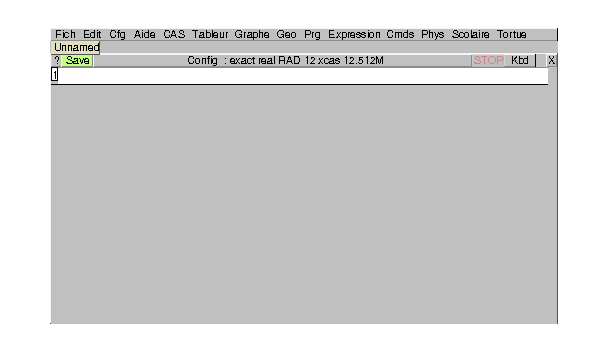
\includegraphics[width=\textwidth]{demarr1}
%\includegraphics[width=\textwidth]{ecran1}
}
Vous pouvez la redimensionner. De haut en bas  cette interface
fait appara\^\i tre~:
\begin{itemize}
\item
une barre de menu cliquable~: \verb|Fich|, \verb|Edit|,
\verb|Cfg|, \verb|Aide|, \verb|CAS|,\verb|Expression|,
\verb|Cmd|,\verb|Prg|,
 \verb|Graphic|, \verb|Geo|,\verb|Tableur|,\ldots
\index{menus}
\item
un onglet indiquant le nom de la session, ou {\tt Unnamed} si la session n'a 
pas encore \'et\'e sauvegard\'ee (on peut ouvrir plusieurs sessions en 
parall\`ele et donc avoir plusieurs onglets repr\'esentant ces sessions),
\item une zone de gestion de la session avec :
\begin{itemize}
\item un bouton \verb|?| pour ouvrir l'index de l'aide,
\item une barre-bouton \verb|Save| pour sauvegarder la session, 
\item un bouton affichant la configuration du CAS
\verb|Config: exact real ...| et permettant de la modifier,
\item un bouton rouge \verb|STOP| permettant d'interrompre un calcul trop long,
\item un bouton \verb|Kbd| pour faire apparaitre un clavier ressemblant \`a 
celui d'une calculatrice (on peut le voir ci-dessus). Il peut faciliter vos 
saisies, peut faire afficher une fen\^etre de messages avec touche 
{\tt Kbd->msg} (ou avec le menu {\tt Cfg->Montrer->msg}) et afficher le bandeau 
des commandes avec la touche {\tt Kbd->cmds} (ou avec le menu 
{\tt Cfg->Montrer->bandeau}) 
\item  un bouton \verb|x| pour fermer la session,
\end{itemize}
\item
une zone rectangulaire blanche num\'erot\'ee 1 (premi\`ere ligne
de commande) dans laquelle vous pouvez taper
votre premi\`ere commande (cliquez si n\'ecessaire pour faire
apparaitre le curseur dans
cette ligne de commande)~: \verb|1+1|, suivi de la touche
"Entr\'ee" ("Enter" ou "Return" selon les claviers).
Le r\'esultat appara\^it au-dessous, et une nouvelle ligne de commande
s'ouvre, num\'erot\'ee 2. 
\end{itemize}
Vous pouvez modifier l'aspect de l'interface et sauvegarder vos
modifications pour les utilisations futures (menu \verb|Cfg|).

Vous n'avez pour l'instant qu'\`a
entrer des commandes dans les lignes de commandes successives. 
Si vous utilisez la
version html de ce cours, vous pouvez copier-coller les commandes
propos\'ees depuis votre navigateur. 
Chaque ligne de commande saisie est ex\'ecut\'ee par la
touche "Entr\'ee". Essayez par exemple d'ex\'ecuter les
commandes suivantes :
\begin{verbatim}
1/3+1/4
sqrt(2)^5
solve(a*x^2+b*x+c,x)
50!
\end{verbatim}
Toutes les commandes sont gard\'ees en m\'emoire.
Vous pouvez donc remonter dans l'historique de votre session pour faire 
afficher \`a nouveau des commandes ant\'erieures avec {\tt Ctrl+$\uparrow$}
pour par exemple les modifier. Essayez, par exemple, en modifiant les 
commandes pr\'ec\'edentes d'ex\'ecuter aussi~:
\begin{verbatim}
1/3+3/4
solve(a*x+b*x+c,x)
\end{verbatim}
On obtient alors 

\centerline{
%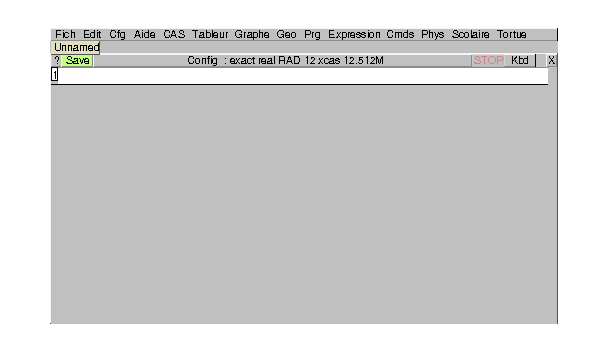
\includegraphics[width=\textwidth]{demarr1}
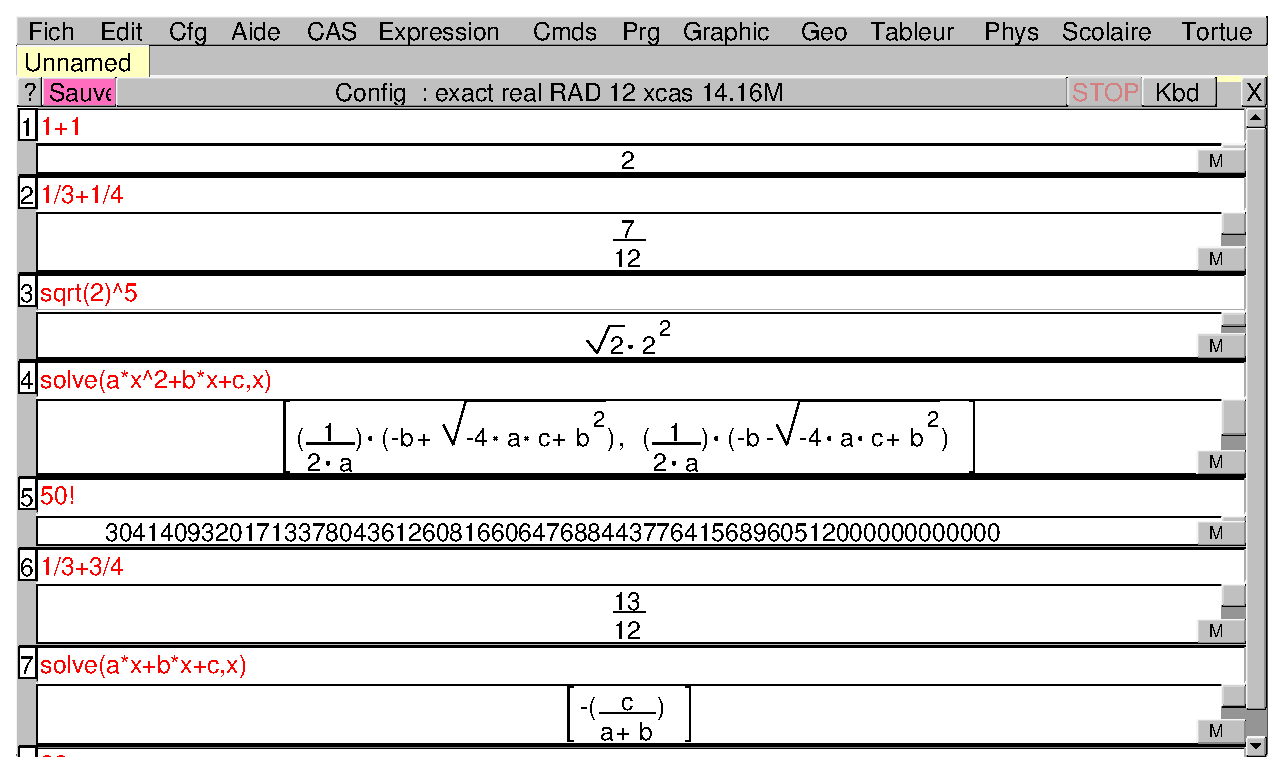
\includegraphics[width=\textwidth]{ecran2}
}
On peut alors voir apparaitre, sur la droite, une barre de scroll permettant de 
se d\'eplacer dans les niveaux de la session et ici par exemple d'avoir 
acc\`es au niveau 8.
Le menu \verb|Edit| vous permet de pr\'eparer des sessions plus
\'elabor\'ees qu'une simple succession de commandes. Vous pouvez
cr\'eer des groupes de lignes de commandes (sections), 
ajouter des commentaires ou fusionner des niveaux en un seul niveau.
%
\subsection{Les commandes et l'aide en ligne}
%
Les commandes sont regroup\'ees par th\`emes dans les
menus du bandeau sup\'erieur~: \verb|CAS|, \verb|Expression|,\verb|Cmds|,
\verb|Prg|, \verb|Graphic|,
\verb|Geo|, \verb|Tableur|,  \verb|Phys|, \verb|Scolaire|, \verb|Tortue|. 
Certains menus sont des menus dit menus "Assistant" parce que les commandes 
sont class\'ees par th\`eme et sont explicit\'ees (menu {\tt CAS}) ou parce 
qu'une boite de dialogue vous demande de 
pr\'eciser les param\`etres de la commande choisie (menu 
{\tt Tableur$\blacktriangleright$Maths} ou menu {\tt Graphic}).\\
Les autres menus contiennent les noms des commandes : 
le menu {\tt Cmds} contient toutes les commandes de calcul formel, 
le menu {\tt Prg} contient toutes les commandes que l'on utilise en  
programmation,
le menu {\tt Geo} contient toutes les commandes de g\'eom\'etrie...
Lorsqu'on s\'electionne une commande dans un menu, 
\begin{itemize}
\item soit une boite de dialogue s'ouvre vous permettant de sp\'ecifier
les arguments de la commande (par exemple pour tracer une courbe
depuis le menu \verb|Graphic| ou pour faire des statistiques depuis le menu 
{\tt Tableur$\blacktriangleright$Maths},
\item soit la commande est recopi\'ee dans la ligne de commande. Pour connaitre
la syntaxe de cette commande, appuyez sur le bouton \verb|?| en haut \`a 
gauche, ou faites afficher la zone de \verb|Messages| (en utilisant le menu 
\verb|Cfg->Montrer->msg|). \\
Vous pouvez aussi :
\begin{itemize}
\item ouvrir l'index de l'aide \`a la commande s\'electionn\'ee
(cela est  automatique si on  a cocher la case 
\verb|Aide index automatique| dans le menu de configuration 
g\'en\'erale : \verb|Cfg|->\verb|Configuration generale|). Il faut alors 
cliquer sur le bouton {\tt OK} pour que la commande soit recopi\'ee dans la 
ligne de commande \`a condition que le curseur soit dans une ligne de 
commande.\\utoriel.tex
Vous pouvez aussi cliquer sur le bouton
\verb|Details| pour afficher la page du manuel correspondant \`a la commande
dans votre navigateur. 

\item  ouvrir automatiquement la page correspondante du manuel dans votre 
navigateur, en cochant la case \verb|Aide HTML automatique| dans le menu de 
configuration  g\'en\'erale (\verb|Cfg|-> \verb|Configuration generale|).
\end{itemize}
\end{itemize}
Le menu \verb|Aide| contient les diff\'erentes formes d'aide possible~:
un guide de l'utilisateur (interface), un guide de r\'ef\'erence
(\verb|Manuels->Calcul formel|, aide detaill\'ee sur chaque commande), 
un \verb|Index| (liste des commandes class\'ees par ordre 
alphab\'etique avec une ligne d'entr\'ee permettant de se d\'eplacer
facilement) et une recherche par mots clefs.
\index{aide en ligne}
\index{help@{\verb+help+}}

Si vous connaissez d\'ej\`a le nom d'une commande et que vous d\'esirez
v\'erifier sa syntaxe (par exemple \verb|factor|), vous pouvez
saisir le d\'ebut du nom de commande 
(disons \verb|fact|) puis taper sur la touche de tabulation
(situ\'ee \`a gauche de la touche A sur un clavier
fran\c{c}ais) ou cliquer sur le bouton \verb|?| en haut \`a gauche. 
L'index des commandes appara\^\i t alors dans une fen\^etre, positionn\'e 
\`a la premi\`ere compl\'etion possible, avec une aide succinte sur chaque
commande. 
Par exemple, vous voulez factoriser un polyn\^ome, vous supposez que le nom de
commande commence par \verb|fact|, vous tapez donc \verb|fact| puis
la touche de tabulation, vous s\'electionnez \`a la souris
\verb|factor| (ou un des exemples) puis vous cliquez sur OK.

Vous pouvez aussi saisir \verb|?factor| pour avoir l'aide succinte
en r\'eponse. Si le nom que vous avez saisi n'est pas reconnu, des
commandes proches vous sont sugg\'er\'ees.

%
\subsection{Entrer des commandes}
%
L'ex\'ecution d'une ligne se fait simplement par la touche "Entr\'ee". 
Si on ne souhaite pas afficher le r\'esultat, on termine la ligne de commande
par \verb|:;| et on valide avec "Entr\'ee".
On peut \'editer plusieurs commandes \`a la file avant leur ex\'ecution
\`a condition de les s\'eparer par un point-virgule.

Au d\'ebut, de nombreuses erreurs proviennent d'une
mauvaise traduction des math\'ematiques~: {\tt Xcas} ne peut pas les comprendre
telles que vous les \'ecrivez. Votre clavier vous
permet de taper $ax^2+bx+c$, mais votre ordinateur ne peut pas
comprendre que vous souhaitez \'elever $x$ au carr\'e, le multiplier
par $a$, etc\ldots~ Vous devez sp\'ecifier chaque op\'eration, et la
syntaxe correcte est \verb|a*x^2+b*x+c|.  
La multiplication doit \^etre not\'ee par une \'etoile 
dans les commandes, mais est not\'ee par un point dans
les r\'eponses. Nous insistons sur le fait que pour {\tt Xcas}, \verb|ax| est 
une variable dont le nom comporte deux lettres, et pas le produit de \verb|a|
par \verb|x|.

\begin{center}
\begin{tabular}{|ll|}
\hline
\multicolumn{2}{|c|}{\bf Op\'erations}\\
\hline\hline
\verb|+|& addition\\
\verb|-|& soustraction \\
\verb|*|& mutiplication  \\
\verb|/|& division\\
\verb|^|& puissance  \\
\hline
\end{tabular}
\end{center}
\index{addition}
\index{soustraction}
\index{multiplication}
\index{division}
\index{puissance}

Modulo quelques pr\'ecautions, l'\'ecriture des formules est assez
directe. Les parenth\`eses ont le sens 
usuel pour sp\'ecifier l'ordre des op\'erations. Les crochets 
sont r\'eserv\'es aux listes et aux indices.
Les priorit\'es entre op\'erations sont standard 
(la multiplication est prioritaire sur l'addition, la puissance sur
la multiplication). Par exemple~:
\index{priorit\'es}
\index{parenth\`eses}
%
\begin{itemize}
\item
\verb|2*a+b| retourne $2\cdot a+b$
\item
\verb|a/2*b| retourne $\displaystyle \frac{a\cdot b}{2}$\\
\item
\verb|a/2/b| retourne $\displaystyle \frac{a}{\displaystyle \frac{2}{b}}$
\item
\verb|normal(a/2/b)| retourne $\displaystyle \frac{a}{2\cdot b}$
\item
\verb|a^2*b| retourne $a^2\cdot b$
\end{itemize}
Dans le doute, il est toujours prudent de mettre des parenth\`eses 
pour s'assurer que l'ordre des op\'erations est celui souhait\'e.

Les commandes sont num\'erot\'ees, ainsi que les r\'eponses,
mais, si vous avez modifi\'e une ligne de commande, celle-ci
garde le num\'ero qu'elle avait. On peut rappeler par \verb|ans()| (answer) la 
r\'eponse pr\'ec\'edente c'est \`a dire la r\'eponse de la derni\`ere commande
\'evalu\'ee.
\index{ans@{\verb+ans+}}
%
\section{Les objets du calcul formel}
%
\subsection{Les nombres}
%
\index{nombre!exact}
\index{nombre!approch\'e}
Les nombres peuvent \^etre exacts ou approch\'es.
Les nombres exacts sont les constantes pr\'ed\'efinies, les entiers, 
les fractions d'entiers et plus g\'en\'eralement toute  expression 
ne contenant que des entiers et des constantes, comme 
\verb|sqrt(2)*e^(i*pi/3)|.
Les nombres approch\'es sont not\'es avec la notation scientifique 
standard~: partie enti\`ere suivie du point de s\'eparation 
et partie fractionnaire (\'eventuellement
suivie de \verb|e| et d'un exposant).
Par exemple, \verb|2| est un entier exact, 
\verb|2.0| est la version approch\'ee du m\^eme
entier; \verb|1/2| est un  rationnel, \verb|0.5| 
est la version approch\'ee du m\^eme
rationnel.
{\tt Xcas} peut g\'erer des nombres entiers en pr\'ecision arbitraire~: 
essayez de taper \verb|500!| et comptez le nombre de chiffres 
de la r\'eponse.

On passe d'une valeur exacte \`a une valeur approch\'ee par
\verb|evalf|, on transforme une valeur approch\'ee en un rationnel
exact par \verb|exact|
\index{exact@{\verb+exact+}}
\index{evalf@{\verb+evalf+}}
Les calculs sont effectu\'es en mode exact si tous les nombres qui
interviennent sont exacts. Ils sont effectu\'es en mode approch\'e si
un des nombres est approch\'e. Ainsi
\verb|1.5+1| renvoie un nombre approch\'e alors que \verb|3/2+1| 
renvoie un nombre exact.
\begin{verbatim}
sqrt(2)
evalf(sqrt(2))
sqrt(2)-evalf(sqrt(2))
exact(evalf(sqrt(2)))*10^9
exact(evalf(sqrt(2)*10^9))
\end{verbatim} 
\index{sqrt@{\verb+sqrt+}}
\index{precision@pr\'ecision}
Pour les nombres r\'eels approch\'es, la pr\'ecision par d\'efaut est
proche de 14 chiffres significatifs (la pr\'ecision relative est de 53
ou 45 bits pour les r\'eels flottants normalis\'es selon les versions de Xcas). 
Elle peut \^etre augment\'ee, en
donnant le nombre de d\'ecimales d\'esir\'e
comme second argument de \verb|evalf|.
\begin{verbatim}
evalf(sqrt(2),50)
evalf(pi,100)
\end{verbatim}
On peut aussi changer la pr\'ecision par d\'efaut pour tous les
calculs en modifiant
\index{digits@{\verb+Digits+}}
la variable \verb|Digits|.
\begin{verbatim}
Digits:=50
evalf(pi)
evalf(exp(pi*sqrt(163)))
\end{verbatim}

\index{i@{\verb+i+}}
La lettre \verb|i| est r\'eserv\'ee \`a $\sqrt{-1}$ et ne peut \^etre
r\'eaffect\'ee~; en particulier on ne peut pas l'utiliser comme indice
de boucle.
\begin{verbatim}
(1+2*i)^2
(1+2*i)/(1-2*i)
e^(i*pi/3)
\end{verbatim}
\index{nombre!complexe}
\index{infinity@{\verb+infinity+}}
{\tt Xcas} distingue l'infini non sign\'e \verb|infinity| ($\infty$), de
\verb|+infinity| ou \verb|inf| ($+\infty$) et de \verb|-infinity|  
ou \verb|-inf|($-\infty$).
\begin{verbatim}
1/0; (1/0)^2; -(1/0)^2 
\end{verbatim}

\begin{center}
\begin{tabular}{|ll|}
\hline
\multicolumn{2}{|c|}{\bf Constantes pr\'ed\'efinies}\\
\hline\hline
\verb|pi|&$\pi\simeq 3.14159265359$ \\
\verb|e|&$e\simeq 2.71828182846$  \\
\verb|i|&$i=\sqrt{-1}$  \\
\verb|infinity|&$\infty$  \\
\verb|+infinity| ou \verb|inf|&$+\infty$  \\
\verb|-infinity| ou \verb|-inf|&$-\infty$  \\
\hline
\end{tabular}
\end{center}
\index{e@{\verb+e+}}
\index{pi@{\verb+pi+}}
%
\subsection{Les caract\`eres et les cha\^{i}nes}
%
\index{caract\`ere}
\index{cha\^{i}ne}
Une cha\^{i}ne est parenth\'es\'ee par des guillemets ({\tt "}).
Un caract\`ere est une cha\^{i}ne ayant un seul \'el\'ement.
\begin{verbatim}
s:="azertyuiop"
size(s)
s[0]+s[3]+s[size(s)-1]
concat(s[0],concat(s[3],s[size(s)-1]))
head(s)
tail(s)
mid(s,3,2)
l:=asc(s)
ss:=char(l)
string(123)
expr(123)
expr(0123)
\end{verbatim}

\begin{center}
\begin{tabular}{|ll|}
\hline
\multicolumn{2}{|c|}{\bf Cha\^{i}nes}\\
\hline\hline
\verb|asc|&cha\^{i}ne->liste des codes ASCII \\
\verb|char|&liste des codes ASCII->cha\^{i}ne \\
\verb|size|&nombre de caract\`eres \\
\verb|concat| ou \verb|+| &concat\'enation  \\
\verb|mid|&morceau de cha\^{i}ne\\
\verb|head|&premier caract\`ere  \\
\verb|tail|&cha\^{i}ne sans le 1ier caract\`ere\\
\verb|string|&nombre ou expression->cha\^{i}ne  \\
\verb|expr|&cha\^{i}ne->nombre (base 10 ou 8) ou expression  \\
\hline
\end{tabular}
\end{center}%
\subsection{Les variables}
%
\index{variable!formelle}
\index{variable!affect\'ee}
On dit qu'une variable est formelle si elle ne contient aucune valeur~: 
toutes les variables sont formelles tant qu'elles n'ont pas \'et\'e
affect\'ees (\`a une valeur).
\index{affectation}
L'affectation est not\'ee \verb|:=|. Au d\'ebut 
de la session  \verb|a| 
est formelle, elle devient affect\'ee apr\`es l'instruction 
\verb|a:=3|, \verb|a| sera alors remplac\'e par 3 dans tous
les calculs qui suivent, et \verb|a+1| renverra 4. 
{\tt Xcas} conserve tout le contenu de votre session. Si vous voulez que la variable 
\verb|a| apr\`es l'avoir affect\'ee, soit \`a nouveau une variable formelle, il
faut la "vider" par \verb|purge(a)|. Dans les exemples qui suivent, les 
variables utilis\'ees sont suppos\'ees avoir \'et\'e purg\'ees avant chaque
suite de commandes.
\index{purge@{\verb+purge+}}  
\noindent
Il ne faut pas confondre
\begin{itemize}
\item le signe \verb|:=| qui d\'esigne l'affectation
\item le signe \verb|==| qui d\'esigne une \'egalit\'e
  bool\'eenne~: c'est une op\'eration binaire qui retourne 1 ou 0 (1 pour true
qui veut dire Vrai et 0 pour false qui veut dire Faux) 
\item le signe \verb|=| utilis\'e pour d\'efinir une \'equation.
\end{itemize}
\index{egalite@\'egalit\'e}
\index{equation@\'equation}
\begin{verbatim}
a==b
a:=b
a==b
solve(a=b,a)
solve(2*a=b+1,a)
\end{verbatim}
\index{assume@{\verb+assume+}}
\index{hypoth\`ese}
On peut faire certains types d'hypoth\`eses sur une variable avec
la commande \verb|assume|, par exemple \verb|assume(a>2)|. Une
hypoth\`ese est une forme sp\'eciale d'affectation, elle efface
une \'eventuelle valeur pr\'ec\'edemment affect\'ee \`a la variable.
Lors d'un calcul, la variable n'est pas remplac\'ee mais
l'hypoth\`ese sera utilis\'ee dans la mesure du possible, par exemple
\verb|abs(a)| renverra \verb|a| si on fait l'hypoth\`ese \verb|a>2|.
\begin{verbatim}
sqrt(a^2)
assume(a<0)
sqrt(a^2)
assume(n,integer)
sin(n*pi)
\end{verbatim}
\index{subst@{\verb+subst+}}
La fonction \verb|subst| permet de remplacer une variable dans une
expression par un nombre ou une autre expression, 
sans affecter cette variable.
\begin{verbatim}
subst(a^2+1,a=1)
subst(a^2+1,a=sqrt(b-1))
a^2+1
\end{verbatim} 

{\bf Remarque}~: pour stocker une valeur dans une variable par r\'ef\'erence,
par exemple pour modifier une valeur dans une liste (un vecteur, une
matrice), sans recr\'eer une nouvelle liste mais en modifiant
en place la liste existante, on utilise l'instruction \verb|=<|
au lieu de \verb|:=|.
Cette instruction est plus rapide que l'instruction \verb|:=|, car
elle \'economise le temps de copie de la liste.
%
\subsection{Les expressions}
%
\index{expression}
Une expression est une combinaison de nombres et de variables
reli\'es entre eux par des op\'erations~: par exemple 
\verb|x^2+2*x+c|. 

Lorsqu'on valide une commande, {\tt Xcas}
remplace les variables par leur valeur si elles en ont une,
et ex\'ecute les op\'erations. 
\begin{verbatim}
(a-2)*x^2+a*x+1
a:=2
(a-2)*x^2+a*x+1
\end{verbatim}
\index{simplifications automatiques}
Certaines op\'erations de simplification sont ex\'ecut\'ees
automatiquement lors d'une \'evaluation~:
\begin{itemize}
\item les op\'erations sur les entiers et sur les 
fractions, y compris la mise
sous forme irr\'eductible
\item les simplifications triviales comme $x+0=x$,
$x-x=0$, $x^1=x$\ldots
\item quelques formes trigonom\'etriques comme 
$\cos(-x)=\cos(x)$, $\cos(\pi/4)=\sqrt{2}/2$, $\tan(\pi/4)=1$\ldots
\end{itemize}
Nous verrons dans la section suivante comment obtenir plus de simplifications.
%
\subsection{D\'evelopper et simplifier}
%
\index{developper@d\'evelopper}
\index{simplifier@simplifier}
En-dehors des r\`egles de la section pr\'ec\'edente,
il n'y a pas de simplification syst\'ematique. 
Il y a deux raisons \`a cela. La premi\`ere est que les 
simplifications non triviales sont parfois
co\^uteuses en temps, et le choix d'en faire ou non est laiss\'e 
\`a l'utilisateur~;
la deuxi\`eme est qu'il y a en g\'en\'eral plusieurs mani\`eres de
simplifier une m\^eme expression, selon l'usage que l'on veut en
faire. 
Les principales commandes pour transformer une expression 
sont les suivantes~:
\begin{itemize}
\item
\index{expand@{\verb+expand+}}
\verb|expand|~: d\'eveloppe une expression en tenant compte 
uniquement de la distributivit\'e de la multiplication sur l'addition et
du d\'eveloppement des puissances enti\`eres.
\item
\index{normal@{\verb+normal+}}
\index{ratnormal@{\verb+ratnormal+}}
\verb|normal| et \verb|ratnormal|~: 
d'un bon rapport temps d'ex\'ecution-simplification, elles
\'ecrivent une fraction rationnelle (rapport de deux polyn\^omes)
sous forme de fraction irr\'eductible d\'evelopp\'ee; \verb|normal|
tient compte des nombres alg\'ebriques (par exemple comme \verb|sqrt(2)|)
mais pas \verb|ratnormal|. Les deux ne tiennent pas compte des relations
entre fonctions transcendantes (par exemple comme \verb|sin| et \verb|cos|).
\item 
\index{factor@{\verb+factor+}}
\verb|factor|~: un peu plus lente que les pr\'ec\'edentes, elle
\'ecrit une fraction sous forme irr\'eductible factoris\'ee.
\item 
\index{simplify@{\verb+simplify+}}
\verb|simplify|~: elle essaie de se ramener \`a
des variables alg\'ebriquement ind\'ependantes avant d'appliquer
\verb|normal|. Ceci est plus co\^uteux en temps et "aveugle" (on
ne contr\^ole pas les r\'e\'ecritures interm\'ediaires).
Les simplifications faisant intervenir des extensions
alg\'ebriques (par exemple des racines carr\'ees) 
n\'ecessitent parfois deux appels et/ou des hypoth\`eses (\verb|assume|)
pour enlever des valeurs absolues avant d'obtenir la simplification
souhait\'ee.
\item 
\index{tsimplify@{\verb+tsimplify+}}
\verb|tsimplify| essaie de se ramener \`a des variables 
alg\'ebriquement ind\'ependantes mais sans appliquer \verb|normal|
ensuite.
\end{itemize}
Dans le menu \verb|Expression| du bandeau sup\'erieur, les sous-menus sont
des menus de r\'e\'ecriture et contiennent d'autres fonctions, pour des 
transformations plus ou moins sp\'ecialis\'ees.  
\begin{verbatim}
b:=sqrt(1-a^2)/sqrt(1-a)
ratnormal(b)
normal(b)
tsimplify(b)
simplify(b)
simplify(simplify(b))
assume(a<1)
simplify(b)   
simplify(simplify(b))
\end{verbatim}
\index{convert@{\verb+convert+}}
La fonction \verb|convert| permet de passer d'une expression \`a une
autre \'equivalente, sous un format qui est sp\'ecifi\'e par le
deuxi\`eme argument. 
\begin{verbatim}
convert(exp(i*x),sincos)
convert(1/(x^4-1),partfrac)
convert(series(sin(x),x=0,6),polynom)
\end{verbatim}

\begin{center}
\begin{tabular}{|ll|}
\hline
\multicolumn{2}{|c|}{\bf Transformations}\\
\hline\hline
\verb|simplify|& simplifier\\
\verb|tsimplify|& simplifier (moins puissant)\\
\verb|normal|& forme normale\\
\verb|ratnormal|& forme normale (moins puissant)\\
\verb|expand|& d\'evelopper\\
\verb|factor|& factoriser\\
\verb|assume|& rajout d'hypoth\`eses\\
\verb|convert|& transformer en un format sp\'ecifi\'e\\
\hline
\end{tabular}
\end{center}
%
\subsection{Les fonctions}
%
De nombreuses fonctions sont d\'ej\`a d\'efinies dans {\tt Xcas}, en
particulier les fonctions classiques. Les plus courantes figurent dans
le tableau ci-apr\`es; pour les autres, voir le menu \verb|Cmds->Reel->Special|.\\

Sinon l'utilisateur peut d\'efinir ses propre fonctions, par exemple :
\begin{itemize}
\item D\'efinition d'une fonction d'une variable :\\
{\tt f(x):=x*exp(x)} ou\\
{\tt f:=x->x*exp(x)} ou\\
{\tt f:=unapply(x*exp(x),x)}
\item D\'efinition de sa d\'eriv\'ee :\\
{\tt g:=function\_diff(f)} ou \\
{\tt g:=unapply(diff(f(x),x),x)})\\
{\bf ATTENTION} {\tt g(x):=diff(f(x),x)} N'EST PAS VALABLE ! car ce qui est 
\`a droite de {\tt :=} n'est pas \'evalu\'e lors de la d\'efinition....il
faut utiliser {\tt unapply}.
\item D\'efinition d'une fonction de 2 variables :\\
{\tt h(r,t):=(r*exp(t),r*t)} ou\\
{\tt h:=(r,t)->(r*exp(t),r*t);}
\item D\'efinition \`a partir d'une fonction de 2 variables, d'une fonction qui
\`a 1 variable fait correspondre une fonction:\\
{\tt k(t):=unapply(h(r,t),r)}\\
{\bf ATTENTION} Ici {\tt k(t)} est une fonction de la variable {\tt r}
qui \`a {\tt r} fait 
correspondre {\tt h(r,t)}. On a par exemple : {\tt k(1)(2)=(2*exp(1),2)}. L\`a aussi, il faut 
utiliser {\tt unapply}.
\end{itemize}

\begin{center}
\begin{tabular}{|ll|}
\hline
\multicolumn{2}{|c|}{\bf Fonctions classiques}\\
\hline\hline
\verb|abs| & valeur absolue\\
\verb|sign| & signe (-1,0,+1)\\
\verb|max| & maximum\\
\verb|min| & minimum\\
\verb|round| & arrondi \\
\verb|floor| & partie enti\`ere (plus grand entier $\leq$)\\
\verb|frac| & partie fractionnaire\\
\verb|ceil| & plus petit entier $\geq $\\
\hline
\verb|re| & partie r\'eelle\\
\verb|im| & partie imaginaire\\
\verb|abs| & module\\
\verb|arg| & argument\\
\verb|conj| & conjugu\'e\\
\verb|affixe| & affixe\\
\verb|coordonees| & coordonn\'ees\\
\hline
\verb|factorial ou !| & factorielle\\
\verb|sqrt| & racine carr\'ee\\
\verb|exp| & exponentielle\\
\verb|log| & logarithme naturel\\
\verb|ln| & logarithme naturel\\
\verb|log10| & logarithme en base 10\\
\hline
\verb|sin| & sinus\\
\verb|cos| & cosinus\\
\verb|tan| & tangente\\
\verb|cot| & cotangente\\
\verb|asin| & arc sinus\\
\verb|acos| & arc cosinus\\
\verb|atan| & arc tangente\\
\hline
\verb|sinh| & sinus hyperbolique\\
\verb|cosh| & cosinus hyperbolique\\
\verb|tanh| & tangente hyperbolique\\
\verb|asinh| & argument sinus hyperbolique\\
\verb|acosh| & argument cosinus hyperbolique\\
\verb|atanh| & argument tangente hyperbolique\\
\hline
\end{tabular}
\end{center}
\index{abs@{\verb+abs+}}
\index{valeur absolue}
\index{sign@{\verb+sign+}}
\index{signe}
\index{max@{\verb+max+}}
\index{maximum}
\index{min@{\verb+min+}}
\index{minimum}
\index{round@{\verb+round+}}
\index{arrondi}
\index{floor@{\verb+floor+}}
\index{ceil@{\verb+ceil+}}
\index{partie enti\`ere}
\index{frac@{\verb+frac+}}
\index{partie fractionnaire}
\index{re@{\verb+re+}}
\index{partie r\'eelle}
\index{im@{\verb+im+}}
\index{partie imaginaire}
\index{conj@{\verb+conj+}}
\index{conjugu\'e}
\index{affixe@{\verb+affixe+}}
\index{affixe}
\index{coordonn\'ees@{\verb+coordonnees+}}
\index{coordonn\'ees}
\index{factorial@{\verb+factorial+}}
\index{factorielle}
\index{sqrt@{\verb+sqrt+}}
\index{racine carr\'ee}
\index{exp@{\verb+exp+}}
\index{log@{\verb+log+}}
\index{ln@{\verb+ln+}}
\index{logarithme!naturel}
\index{logarithme!en base 10}
\index{log10@{\verb+log10+}}
\index{sin@{\verb+sin+}}
\index{sinus}
\index{cos@{\verb+cos+}}
\index{cosinus}
\index{tan@{\verb+tan+}}
\index{tangente}
\index{tan@{\verb+cot+}}
\index{cotangente}
\index{sinh@{\verb+sinh+}}
\index{sinus!hyperbolique}
\index{cosh@{\verb+cosh+}}
\index{cosinus!hyperbolique}
\index{tanh@{\verb+tanh+}}
\index{tangente!hyperbolique}
\index{asin@{\verb+asin+}}
\index{arc!sinus}
\index{acos@{\verb+acos+}}
\index{arc!cosinus}
\index{atan@{\verb+atan+}}
\index{arc!tangente}
\index{asinh@{\verb+asinh+}}
\index{argument!sinus hyperbolique}
\index{acosh@{\verb+acosh+}}
\index{argument!cosinus hyperbolique}
\index{atanh@{\verb+atanh+}}
\index{argument!tangente hyperbolique}
Pour cr\'eer une nouvelle fonction, il faut la d\'eclarer \`a l'aide 
d'une expression contenant la variable. 
Par exemple l'expression $x^2-1$ est 
d\'efinie par \verb|x^2-1|. Pour la transformer en la fonction $f$ qui
\`a $x$ associe $x^2-1$, trois possibilit\'es existent~:
\begin{verbatim}
f(x):= x^2-1
f:=x->x^2-1
f:=unapply(x^2-1,x)

f(2); 
f(a^2);
\end{verbatim}
\index{fonction!d\'efinition d'une}
\index{fonction}
\index{expression}
\index{unapply@{\verb+unapply+}}
Si \verb|f| est une fonction d'une variable et \verb|E| est une
expression, \verb|f(E)| est une autre expression.
Il est essentiel de ne pas confondre fonction et expression.
Si on d\'efinit : \verb|E:=x^2-1|, alors la variable \verb|E| 
contient l'expression $x^2-1$. Pour avoir la valeur de cette
expression en $x=2$ il faut 
\'ecrire \verb|subst(E,x=2)| et non \verb|E(2)|
car \verb|E| n'est pas une fonction.
Lorsqu'on d\'efinit une fonction,
le membre de droite de l'affectation n'est pas \'evalu\'e.
Ainsi l'\'ecriture \verb|E:=x^2-1; f(x):=E|
d\'efinit la fonction $f: x \mapsto E$ car \verb|E| n'est pas \'evalu\'e.
Par contre \verb|E:= x^2-1; f:=unapply(E,x)| d\'efinit bien la
fonction $f: x\mapsto x^2-1$ car \verb|E| est \'evalu\'e.

\index{fonction!composition des}
\index{compos\'ee}
On peut ajouter et multiplier des fonctions,
par exemple \verb|f:=sin*exp|. Pour composer des fonctions, on utilise 
l'op\'erateur \verb|@| et pour composer plusieurs fois une fonction 
avec elle-m\^eme, on utilise l'op\'erateur \verb|@@|.
\begin{verbatim}
f:=x->x^2-1;
(f@f)(2);
(f@sqrt)(a);
f1:=f@sin
f2:=f@f
f3:=f@@3
f1(a)
f2(a)
f3(a)
\end{verbatim} 
%
On peut d\'efinir des fonctions de plusieurs variables \`a valeurs dans 
$\mathbb R$ comme :\\
\verb|f(x,y):=x+2*y| \\
et des fonctions de plusieurs variables \`a valeurs dans $\mathbb R^p$
par exemple :\\
\verb|f(x,y):=(x+2*y,x-y)| 

% Attention : on peut aussi d\'efinir  \verb|f(x,y)| comme un vecteur mais il 
% faut mettre des accolades.
% Par exemple, on tape \verb|f(x,y):={[x+2*y,x-y]}|. Les accolades sont  n\'ecessaires car sans elles, {\tt Xcas} comprendrait \verb|[x+2*y,x-y]| comme un programme 
% ayant deux instructions \verb|x+2*y;| et \verb|x-y;| 
% et $f$ ne renverrait que la derni\`ere instruction. 
%
\subsection{Listes, s\'equences, ensembles}
%
\index{liste}
\index{sequence@s\'equence}
\index{ensemble}
{\tt Xcas} distingue plusieurs sortes de collections d'objets, 
s\'epar\'es par des virgules~: 
\begin{itemize}
\item les listes (entre crochets)
\item  les s\'equences (entre parenth\`eses) 
\item  les ensembles (entre pourcentage-accolades)
\end{itemize}
\begin{verbatim}
liste:=[1,2,4,2]
sequence:=(1,2,4,2)
ensemble:=%{1,2,4,2%}
\end{verbatim}
Les listes peuvent contenir des listes (c'est le cas des matrices), 
alors que les s\'equences sont plates (un \'el\'ement d'une s\'equence
ne peut pas \^etre une s\'equence). Dans un ensemble,
l'ordre n'a pas d'importance et chaque objet est unique. 
Il existe une autre structure, appel\'ee table, dont nous
reparlerons plus loin.

Il suffit de mettre une s\'equence entre crochets pour en faire une liste
ou entre accolades pr\'ec\'ed\'ees de \verb|%| pour en faire un ensemble.
On passe d'une liste \`a sa s\'equence associ\'ee par \verb|op|, 
d'une s\'equence \`a sa liste associ\'ee en la mettant entre crochets
ou avec la fonction \verb|nop|.
Le nombre d'\'el\'ements d'une liste est donn\'e par \verb|size| 
(ou \verb|nops|).
\index{op@{\verb+op+}}
\index{nop@{\verb+nop+}}
\index{nops@{\verb+nops+}}
\index{size@{\verb+size+}}
\index{nombre!d'\'el\'ements}
\begin{verbatim}
se:=(1,2,4,2)
li:=[se]
op(li)
nop(se)
nops(se)
%{se%}
size([se])
size(%{se%})
\end{verbatim}
\index{it\'eration}
\index{seq@{\verb+seq+}}
\index{makelist@{\verb+makelist+}}
Pour fabriquer une liste ou une s\'equence, on utilise des commandes
d'it\'eration comme \verb|$| %$ 
ou \verb|seq| (qui it\`erent une
expression) ou \verb|makelist| (qui d\'efinit une liste \`a l'aide d'une 
fonction).  
\begin{verbatim}
1$5
k^2 $ (k=-2..2)
seq(k^2,k=-2..2)
seq(k^2,k,-2..2)
[k^2$(k=-2..2)]
seq(k^2,k,-2,2)
seq(k^2,k,-2,2,2)
makelist(x->x^2,-2,2)
seq(k^2,k,-2,2,2)
makelist(x->x^2,-2,2,2)
\end{verbatim}
\index{NULL@{\verb+NULL+}}
\index{liste!vide}
\index{sequence@s\'equence!vide}
La s\'equence vide est not\'ee \verb|NULL|, la liste vide
\verb|[]|. Pour ajouter un \'el\'ement \`a une s\'equence il suffit
d'\'ecrire la s\'equence et l'\'el\'ement s\'epar\'es par une virgule. 
\index{append@{\verb+append+}}
Pour ajouter un
\'el\'ement \`a une liste on utilise \verb|append|.
On acc\`ede \`a un \'el\'ement d'une liste ou d'une s\'equence gr\^ace 
\`a son indice mis entre 
crochets, le premier \'el\'ement \'etant d'indice 0.
\begin{verbatim}
se:=NULL; se:=se,k^2$(k=-2..2); se:=se,1
li:=[1,2]; (li:=append(li,k^2))$(k=-2..2)
li[0],li[1],li[2]
\end{verbatim}

Les polyn\^omes sont souvent d\'efinis par une expression, mais
ils peuvent aussi \^etre repr\'esent\'es 
par la liste de leurs coefficients par ordre
de degr\'e d\'ecroissant, avec comme d\'elimiteurs \verb|poly1[| et \verb|]|.
Il existe aussi une repr\'esentation
pour les polyn\^omes \`a plusieurs variables. Les fonctions
\verb|symb2poly| et \verb|poly2symb| permettent
de passer de la repr\'esentation expression \`a la repr\'esentation
par liste et inversement, 
le deuxi\`eme argument d\'etermine s'il s'agit de polyn\^omes
en une variable (on met le nom de la variable) ou de
polyn\^omes \`a plusieurs variables (on met la liste des variables).

\begin{center}
\begin{tabular}{|ll|}
\hline
\multicolumn{2}{|c|}{\bf S\'equences et listes}\\
\hline\hline
\verb|E$(k=n..m)| &cr\'eer une s\'equence\\
\verb|seq(E,k=n..m)| &cr\'eer une s\'equence\\
\verb|[E$(k=n..m)]| & cr\'eer une liste\\
%$
\verb|makelist(f,k,n,m,p)| & cr\'eer une liste\\
\verb|op(li)| & passer de liste \`a s\'equence\\
\verb|nop(se)| & passer de s\'equence \`a liste\\
\verb|nops(li)| & nombre d'\'el\'ements\\
\verb|size(li)| & nombre d'\'el\'ements\\
\verb|sum| & somme des \'el\'ements\\
\verb|product| & produit des \'el\'ements\\
\verb|cumSum| & sommes cumul\'ees des \'el\'ements\\
\verb|apply(f,li)| & appliquer une fonction aux \'el\'ements d'une liste\\
\verb|map(li,f)| & appliquer une fonction  aux \'el\'ements d'une liste\\
\verb|map(li,f,matrix)| & appliquer une fonction  aux \'el\'ements d'une matrice\\
\verb|poly2symb| & polyn\^ome associ\'e \`a une liste\\
\verb|symb2poly| & coefficients d'un polyn\^ome\\
\hline
\end{tabular}
\end{center}
\index{sum@{\verb+somme+}}
\index{somme}
\index{product@{\verb+product+}}
\index{produit}
\index{cumsum@{\verb+cumSum+}}
\index{sommes cumul\'ees}
\index{apply@{\verb+apply+}}
\index{fonction!appliqu\'ee \`a une liste}
\index{map@{\verb+map+}}
\index{poly2symb@{\verb+poly2symb+}}
\index{symb2poly@{\verb+symb2poly+}}
\index{liste!des coefficients}
%
\subsection{Temps de calcul, place m\'emoire}
%
Le principal probl\`eme du calcul formel est la complexit\'e des 
calculs interm\'ediaires. Elle se traduit \`a la fois par le temps
n\'ecessaire \`a l'ex\'ecution des commandes et par la place m\'emoire
requise. Les algorithmes impl\'ement\'es dans les fonctions
de {\tt Xcas} sont performants, mais ils ne
\index{time@{\verb+time+}}
\index{temps de calcul}
peuvent pas \^etre optimaux dans tous les cas. La fonction \verb|time| 
permet de conna\^\i tre le temps d'ex\'ecution d'une commande (si ce temps
est tr\`es court, {\tt Xcas} ex\'ecute plusieurs fois la commande pour
afficher un r\'esultat plus pr\'ecis). La m\'emoire utilis\'ee 
appara\^\i t dans les versions Unix dans la ligne d'\'etat
(la barre-bouton). Si le temps d'ex\'ecution d'une
commande d\'epasse quelques secondes, il est possible que vous ayez
commis une erreur de saisie. N'h\'esitez pas \`a interrompre
l'ex\'ecution (bouton rouge \verb|STOP| en haut \`a droite, il est
conseill\'e de faire une sauvegarde de votre session auparavant).

\section{Outils pour l'Analyse}
%
\subsection{D\'eriv\'ees}
%
\index{derivee@d\'eriv\'ee!d'une expression}
\index{derivee@d\'eriv\'ee!d'une fonction}
\index{diff@{\verb+diff+}}
\index{functiondiff@{\verb+function_diff+}}
La fonction \verb|diff| permet de calculer la d\'eriv\'ee d'une
expression par rapport \`a une ou plusieurs de ses variables. Pour
d\'eriver une fonction $f$, 
on peut appliquer \verb|diff| \`a l'expression $f(x)$, mais alors le
r\'esultat est une expression. Si on souhaite d\'efinir la fonction
d\'eriv\'ee, il faut utiliser \verb|function_diff|.
\begin{verbatim}
E:=x^2-1; diff(E);
f:=unapply(E,x); diff(f(x));
f1:=function_diff(f);f1(x);
\end{verbatim}
Il ne {\bf faut pas} d\'efinir la fonction d\'eriv\'ee par
\verb|f1(x):=diff(f(x))|, car dans cette d\'efinition, \verb|x| aurait 
deux sens incompatibles~: c'est d'une part la
variable formelle de d\'erivation et d'autre part l'argument
de la fonction \verb|f1|. D'autre part, cette d\'efinition
\'evaluerait \verb|diff| \`a chaque appel de la fonction (car
le membre de droite d'une affectation n'est jamais \'evalu\'e), ce 
qui serait inefficace.\\ Il faut utiliser
\verb|f1:=function_diff(f)|, 
ou
\verb|f1:=unapply(diff(f(x)),x)|.

La fonction \verb|diff| s'applique \`a n'importe quelle combinaison de
variables, et permet de calculer des d\'eriv\'ees partielles
successives.
\index{derivee@d\'eriv\'ee!partielle}
\begin{verbatim}
E:=sin(x*y)
diff(E,x)
diff(E,y)
diff(E,x,y)-diff(E,y,x)
simplify(ans())
diff(E,x$2,y$3)
\end{verbatim}
Si le deuxi\`eme argument de \verb|diff| est une liste, une
liste de d\'eriv\'ees est retourn\'ee. Par exemple pour calculer
le gradient de $\sin(xy)$~:
\verb|diff(sin(x*y),[x,y])| (on peut aussi utiliser \verb|grad|). 
Des commandes particuli\`eres permettent de calculer les  
combinaisons classiques de d\'eriv\'ees partielles.

\begin{center}
\begin{tabular}{|ll|}
\hline
\multicolumn{2}{|c|}{\bf D\'eriv\'ees}\\
\hline\hline
\verb|diff(ex,t)| &d\'eriv\'ee d'une expression par rapport \`a t\\
\verb|function_diff(f)| & fonction d\'eriv\'ee d'une fonction\\
\verb|diff(ex,x$n,y$m)| & d\'eriv\'ees partielles\\
\verb|grad| & gradient\\ 
\verb|divergence| & divergence\\
\verb|curl| & rotationnel\\
\verb|laplacian| & laplacien\\
\verb|hessian| & matrice hessienne\\
\hline
\end{tabular}
\end{center}
\index{grad@{\verb+grad+}}
\index{gradient}
\index{divergence@{\verb+divergence+}}
\index{divergence}
\index{curl@{\verb+curl+}}
\index{rotationnel}
\index{laplacian@{\verb+laplacian+}}
\index{laplacien}
\index{hessian@{\verb+hessian+}}
\index{matrice!hessienne}
%
\subsection{Limites et d\'eveloppements limit\'es}
%
La fonction  \verb|limit| calcule les limites finies ou
infinies, quand elles existent. On peut demander une limite 
\`a gauche ou \`a droite \`a l'aide d'un quatri\`eme argument (+1 ou -1). 
Quand la fonction d\'epend d'un
param\`etre, la limite obtenue peut d\'ependre des hypoth\`eses
faites, avec la fonction {\tt assume}, sur ce param\`etre. 
\index{limit@{\verb+limit+}}
\index{limite}
\index{limite!\`a droite}
\index{limite!\`a gauche}
\begin{verbatim}
limit(1/x,x,0)
limit(1/x,x,0,1)
limit(1/x,x,0,-1)
limit(a/x,x,0,1)
assume(a>0)
limit(a/x,x,0,1)
\end{verbatim}
Pour les d\'eveloppements limit\'es,
deux fonctions sont disponibles, \verb|series| et \verb|taylor|. La
diff\'erence est que l'ordre du d\'eveloppement doit \^etre
sp\'ecifi\'e pour \verb|series|, il est \'egal \`a 6 par d\'efaut
pour \verb|taylor|. 
\index{developpement@d\'eveloppement limit\'e}
\index{series@{\verb+series+}}
\index{taylor@{\verb+taylor+}}

L'ordre du d\'eveloppement limit\'e demand\'e est utilis\'e par 
{\tt Xcas} en interne pour faire ses d\'eveloppements. En cas de 
simplifications, l'ordre du d\'eveloppement obtenu pourra \^etre inf\'erieur, 
il faudra alors recommencer le calcul avec un ordre plus grand. L'expression
retourn\'ee est constitu\'ee du polyn\^ome de Taylor, plus un reste
dans lequel appara\^\i t une fonction \verb|order_size| qui est telle que
pour tout $a>0$, $x^a$\verb|order_size|($x$) tend vers $0$
quand $x$ tend vers $0$. Pour supprimer le reste et ne garder
que le polyn\^ome de Taylor, on peut utiliser \verb|convert| avec l'option 
{\tt polynom}.
\begin{verbatim}
taylor(1/(x^2+1),0)
taylor(1/(x^2+a^2),x=0)
series(1/(x^2+1),0,11)
series(1/(x^2+1),+infinity,11)
series(tan(x),pi/4,3)
series(sin(x)^3/((1-cos(x))*tan(x)),0,4)
series(sin(x)^3/((1-cos(x))*tan(x)),0,6)
series(tan(sin(x))-sin(tan(x)),0,13)
convert(ans(),polynom)
series(f(x),0,3)
g:=f@f; series(g(x),0,2)
\end{verbatim}

\begin{center}
\begin{tabular}{|ll|}
\hline
\multicolumn{2}{|c|}{\bf Limites et d\'eveloppements limit\'es}\\
\hline\hline
\verb|limit(ex,x,a)| & limite en a\\
\verb|limit(ex,x,a,1)| & limite \`a droite en a\\
\verb|limit(ex,x,a,-1)| & limite \`a gauche en a\\
\verb|taylor(ex,a)| & d\'eveloppement limit\'e en $a$ ordre 6\\
\verb|series(ex,a,n)| & d\'eveloppement limit\'e en $a$ ordre $n$\\
\hline
\end{tabular}
\end{center}

%
\subsection{Primitives et int\'egrales}
%
\index{int@{\verb+int+}}
\index{primitive}
\index{fonction!primitive d'une}
\index{integrale@int\'egrale}
La fonction \verb|int| calcule une primitive d'une expressionpar rapport \`a 
$x$ ou par rapport \`a la variable donn\'ee en argument. Si
l'expression comporte plusieurs variables, il vaut pr\'eciser la
variable d'int\'egration. Si on ajoute deux arguments $a$ et $b$ 
apr\`es la variable d'int\'egration, on calcule l'int\'egrale sur
l'intervalle $[a,b]$. Eventuellement les
bornes de l'int\'egrale peuvent \^etre des expressions, ce qui permet
de calculer des int\'egrales multiples.
\begin{verbatim}
int(x^2-1)
int(x^2-1,x,-1,1)
int(x*y,x)
int(x*y,y,0,x)
int(int(x*y,y,0,x),x,0,1)
\end{verbatim}
Pour calculer une int\'egrale, un logiciel de calcul formel recherche 
une primitive puis l'\'evalue entre les bornes, afin d'obtenir
une valeur exacte. Dans certains cas, il est inutile de calculer
une primitive, soit parce qu'il n'en existe pas qui s'exprime
avec les fonctions \'el\'ementaires, soit 
parce qu'un calcul num\'erique est plus adapt\'e (par exemple si 
le temps de calcul de la primitive est trop long, si la fonction
pr\'esente des singularit\'es dans l'intervalle d'int\'egration, etc\ldots).
Dans ce cas, on demande une valeur approch\'ee en utilisant
\verb|evalf|, ou bien on utilise directement 
la fonction \verb|romberg|, qui est
appel\'ee par \verb|evalf|.
\index{romberg@{\verb+romberg+}}
\begin{verbatim}
int(exp(-x^2))
int(exp(-x^2),x,0,10)
evalf(int(exp(-x^2),x,0,10))
romberg(exp(-x^2),x,0,10)
ans()/sqrt(pi))
\end{verbatim}

\begin{center}
\begin{tabular}{|ll|}
\hline
\multicolumn{2}{|c|}{\bf Int\'egrales}\\
\hline\hline
\verb|int(E)| &primitive d'une expression\\
\verb|int(E,x,a,b)| & int\'egrale exacte\\
\verb|romberg(E,x,a,b)| & int\'egrale approch\'ee\\
\hline
\end{tabular}
\end{center}
%
\subsection{R\'esolution d'\'equations}
%
\index{equation@\'equation!r\'esolution}
Comme pour les int\'egrales on distingue~:
\begin{itemize}
\item
la r\'esolution exacte qui renvoie toutes les solutions 
lorsque c'est possible (par exemple pour certaines \'equations polynomiales
ou s'y ramenant)
\item
la r\'esolution approch\'ee qui calcule par un algorithme it\'eratif
une valeur proche d'une des solutions.
\end{itemize}
\index{resolution@r\'esolution!exacte}
\index{resolution@r\'esolution!approch\'ee}
La r\'esolution exacte s'effectue \`a l'aide de \verb|solve|, dont le
premier argument est une \'equation. Le membre de droite est
suppos\'e nul s'il n'est pas pr\'ecis\'e. Par 
d\'efaut \verb|solve| ne retourne pas les solutions complexes. 
Pour les obtenir, il faut cocher \verb|Complexe| dans la configuration du CAS
({\tt Cfg->Configuration de CAS} ou sur la barre-bouton 
{\tt Config :exact...})\\ 
Ex\'ecutez les commandes suivantes
avant et apr\`es avoir activ\'e l'option \verb|Complex|. 
\index{solve@{\verb+solve+}}
\begin{verbatim}
solve(x^2-a*x+2,x)
solve(x^2+2,x)
solve(x^3=1,x)
\end{verbatim}
Les racines exactes sont calcul\'ees pour les polyn\^omes de
degr\'e 1 et 2 (les formules de Cardan et Ferrari pour les degr\'es
3 et 4 ne sont pas utilis\'ees, car les solutions obtenues
ne sont pas facilement maniables). En degr\'e sup\'erieur,
la fonction \verb|solve| affiche un message d'erreur et renvoie
une liste vide.

Pour les \'equations trigonom\'etriques, les solutions principales
sont renvoy\'ees. Pour obtenir toutes les solutions, il faut activer
l'option \verb|All_trig_sol|. Comparer les commandes suivantes avec et
sans cette option.
\begin{verbatim}
solve(cos(x),x)
solve(cos(x)+sin(x),x)
\end{verbatim}

La fonction \verb|solve| peut aussi r\'esoudre des syst\`emes
d'\'equations. Le premier argument est la liste des \'equations, le
second est la liste des variables.
\index{syst\`eme!d'\'equations}
\begin{verbatim}
solve([x^2+y-2,x+y^2-2],[x,y])
\end{verbatim}

\index{fsolve@{\verb+fsolve+}}
La fonction de r\'esolution approch\'ee est \verb|fsolve|. Elle
propose en option diff\'erents algorithmes
(menus \verb|Calc->Num_solve_eq | et \verb|Calc->Num_solve_syst|).
 Le plus c\'el\`ebre est
l'algori\-thme de Newton, qui a de multiples variantes. Le principe
g\'en\'eral de tous ces algorithmes est de calculer les termes
successifs d'une suite qui converge vers une solution de l'\'equation
ou du syst\`eme propos\'e. Il faut pour cela choisir selon les cas
un point de d\'epart, ou un intervalle de recherche.
\begin{verbatim}
fsolve((x^5+2*x+1)=0,x,1,newton_solver)
newton(x^5+2*x+1,x,1.0)
newton(x^5+2*x+1,x,1+i)
newton(x^5+2*x+1,x,-1+i)
\end{verbatim}

\begin{center}
\begin{tabular}{|ll|}
\hline
\multicolumn{2}{|c|}{\bf Equations}\\
\hline\hline
\verb|solve(eq,x)| &r\'esolution exacte d'une \'equation\\
\verb|solve([eq1,eq2],[x,y])| &r\'esolution exacte d'un syst\`eme\\
\verb|fsolve(eq,x)| &r\'esolution approch\'ee d'une \'equation\\
\verb|fsolve([eq1,eq2],[x,y])| &r\'esolution approch\'ee d'un syst\`eme\\
\verb|newton| & m\'ethode de Newton\\
\verb|linsolve| & syst\`eme lin\'eaire\\
\verb|proot| & racines approch\'ees d'un polyn\^ome\\
\hline
\end{tabular}
\end{center}
\index{newton@{\verb+newton+}}
\index{linsolve@{\verb+linsolve+}}
\index{proot@{\verb+proot+}}
%
\subsection{Equations diff\'erentielles}
%
\index{equation@\'equation!diff\'erentielle}
Comme dans les deux sections pr\'ec\'edentes, on distingue le
calcul exact, qui n'est pas toujours possible, du calcul
approch\'e. La r\'esolution exacte s'effectue par \verb|desolve|. 
Les d\'eriv\'ees de la fonction inconnue $y$ peuvent s'\'ecrire $y'$,
$y''$, qui sont traduits en \verb|diff(y)|, \verb|diff(diff(y))|.
Si on ne sp\'ecifie pas de condition initiale, le r\'esultat est donn\'e
en fonction de constantes arbitraires.
\begin{verbatim}
desolve(y'=y,y)
desolve(y''+2*y'+y=0,y)
desolve((x^2-1)*y'+2*y=0,y)
\end{verbatim}
Les conditions initiales sont vues comme des \'equations
suppl\'ementaires, qui forment une liste avec l'\'equation 
diff\'erentielle.
\begin{verbatim}
desolve([y'=y,y(0)=1],y)
desolve([y"+2*y'+y=0,y(0)=1],y)
desolve([y"+2*y'+y=0,y(0)=1,y'(0)=1],y)
desolve([y"+2*y'+y=0,y(0)=1,y(1)=0],y)
desolve([(x^2-1)*y'+2*y=0,y(0)=1],y)
desolve((t^2-1)*diff(y(t),t)+2*y(t)=0,y(t))
\end{verbatim}
\index{desolve@{\verb+desolve+}}
\index{odesolve@{\verb+odesolve+}}

La fonction \verb|odesolve| permet de r\'esoudre par des m\'ethodes
num\'eriques une \'equation diff\'erentielle $y'=f(x,y)$ passant par
un point $(x_0,y_0)$. Par exemple
\begin{verbatim}
odesolve(sin(x*y),[x,y],[0,1],2)
\end{verbatim}
permet de calculer $y(2)$ o\`u $y(x)$ est la solution de $y'(x)=\sin(xy)$,
telle que $y(0)=1$.
La fonction \verb|plotode| repr\'esente graphiquement
la solution d'une \'equation diff\'erentielle,
\verb|plotfield| repr\'esente le champ
des tangentes. La fonction 
\verb|interactive_odeplot| repr\'esente le champ
des tangentes et permet de cliquer sur le graphique pour tracer
les solutions passant par les points cliqu\'es.
\begin{verbatim}
plotfield(sin(x*y),[x,y])
plotode(sin(x*y),[x,y],[0,1])
erase()
interactive_plotode(sin(x*y),[x,y])
\end{verbatim}

\begin{center}
\begin{tabular}{|ll|}
\hline
\multicolumn{2}{|c|}{\bf Equations diff\'erentielles}\\
\hline\hline
\verb|desolve| &r\'esolution exacte\\
\verb|odesolve| &r\'esolution approch\'ee\\
\verb|plotode| &trac\'e de trajectoire\\
\verb|plotfield| &trac\'e d'un champ de vecteurs\\
\verb|interactive_plotode| & interface cliquable\\
\hline
\end{tabular}
\end{center}
\index{plotfield@{\verb+plotfield+}}
\index{plotode@{\verb+plotode+}}
\index{interactiveplotode@{\verb+interactive_plotode+}}
%
\section{Outils pour l'Alg\`ebre}

\subsection{Arithm\'etique des entiers}
%
\index{arithm\'etique}
Les op\'erations sur les entiers figurent dans le menu 
\verb|Cmds->Entier|.
\index{modulo}
Les calculs modulo $p$ se font en 
utilisant \verb|% p|. Une fois d\'efini un entier modulo $p$, disons
\verb|a:=3%5|, tous les calculs seront efffectu\'es dans
$\Z/p\Z$~: \verb|a*2| renvoie \verb|1%5| (6 modulo 5),
\verb|1/a| renvoie \verb|2%5|, \ldots~
Pour calculer efficacement les puissances modulo $p$, on peut utiliser ce qui
pr\'ec\`ede, ou la fonction \verb|powermod| ou \verb|powmod|. 
\begin{verbatim}
a:=3%5
a+12
a^4
powermod(3,4,5)
\end{verbatim}
\index{powermod@{\verb+powermod+}}

\begin{center}
\begin{tabular}{|ll|}
\hline
\multicolumn{2}{|c|}{\bf Nombres entiers}\\
\hline\hline
\verb|a%p| & $a$ modulo $p$\\
\verb|powmod(a,n,p)| & $a^n$ modulo $p$\\
\verb|irem| &reste de la division euclidienne\\
\verb|iquo| &quotient de la division euclidienne\\
\verb|iquorem| &quotient et reste\\
\hline
\verb|ifactor| & d\'ecomposition en facteurs premiers\\
\verb|ifactors| & liste des facteurs premiers\\
\verb|idivis| & liste des diviseurs\\
\hline
\verb|gcd| & plus grand diviseur commun\\
\verb|lcm| & plus petit multiple commun\\
\verb|iegcd| & identit\'e de Bezout\\
\verb|iabcuv| & renvoie $[u,v]$ tels que $au+bv=c$\\
\hline
\verb|is_prime| & l'entier est-il premier\\
\verb|nextprime| & prochain entier premier\\
\verb|previousprime| & entier premier pr\'ec\'edent\\
\hline
\end{tabular}
\end{center}
\index{irem@{\verb+irem+}}
\index{reste}
\index{iquo@{\verb+iquo+}}
\index{quotient}
\index{iquorem@{\verb+iquorem+}}
\index{ifactor@{\verb+ifactor+}}
\index{facteurs premiers}
\index{ifactors@{\verb+ifactors+}}
\index{idivis@{\verb+idivis+}}
\index{gcd@{\verb+gcd+}}
\index{PGCD}
\index{lcm@{\verb+lcm+}}
\index{PPCM}
\index{iegcd@{\verb+iegcd+}}
\index{Bezout}
\index{iabcuv@{\verb+iabcuv+}}
\index{isprime@{\verb+is_prime+}}
\index{nombre!premier}
\index{nextprime@{\verb+nextprime+}}
\index{previousprime@{\verb+previousprime+}}
%
\subsection{Polyn\^omes et fractions rationnelles}
%
\index{polyn\^ome}
\index{fraction rationnelle}
Les fonctions de traitement des polyn\^omes sont dans le menu 
\verb|Cmds->Polyn\^omes|. 

On utilise \verb|normal| ou \verb|expand| 
pour d\'evelopper, ou plus g\'en\'eralement mettre une fraction 
sous forme irr\'eductible, et \verb|factor| pour
factoriser. 
\index{normal@{\verb+normal+}}
\index{expand@{\verb+expand+}}
Le r\'esultat d\'epend du corps de nombres dans lequel on
se place. Par d\'efaut il s'agit des rationnels si les coefficients
sont exacts ou des r\'eels sinon. Pour les complexes 
(exacts ou approch\'ees), il
faut activer l'option \verb|Complexe| \`a partir du bouton rappelant la configuration \verb| Config:...|. On peut aussi d\'eclarer les 
coefficients comme des
entiers modulo $p$ pour travailler dans $\Z/p\Z$ (commande \verb|%|) 
ou dans un corps
fini (d\'efini par la commande \verb|GF|). Ex\'ecutez les
commandes suivantes avant et apr\`es avoir activ\'e l'option
\verb|Complexe|.
\begin{verbatim}
P:=x^4-1
factor(P)
gcd(P,x^3-1)
divis(P)
propfrac(x^4/P)
partfrac(4/P)
Q:=(x^4+1)%3
factor(Q)
G:=GF(2,8,['a','G'])
factor(G(a^3)*x^2+1)
genpoly(5,3,x)
genpoly(2,3,x)
genpoly(2*y+5,3,x)
\end{verbatim}

\index{normal@{\verb+normal+}}
\index{expand@{\verb+expand+}}
\index{ptaylor@{\verb+ptayl+}}
\index{peval@{\verb+peval+}}
\index{horner@{\verb+horner+}}
\index{genpoly@{\verb+genpoly+}}
\index{canonicalform@{\verb+canonical_form+}}
\index{coeff@{\verb+coeff+}}
\index{poly2symb@{\verb+poly2symb+}}
\index{symb2poly@{\verb+symb2poly+}}
\index{pcoeff@{\verb+pcoeff+}}
\index{degree@{\verb+degree+}}
\index{lcoeff@{\verb+lcoeff+}}
\index{valuation@{\verb+valuation+}} 
\index{tcoeff@{\verb+tcoeff+}}
\index{partfrac@{\verb+partfrac+}}
\index{decomposition@d\'ecomposition en \'el\'ements simples}
  
\begin{center}
\begin{tabular}{|ll|}
\hline
\multicolumn{2}{|c|}{\bf Polyn\^omes}\\
\hline\hline
\verb|normal| &forme normale (d\'evelopp\'ee et r\'eduite)\\
\verb|expand| &forme d\'evelopp\'ee\\
\verb|ptayl| &forme de Taylor\\
\verb|peval| ou \verb|horner| &\'evaluation en un point par l'algorithme de Horner\\
\verb|genpoly| & polyn\^ome d\'efini par sa valeur en un point\\
\verb|canonical_form| & trin\^ome sous forme canonique\\
\hline
\verb|coeff| &(liste des) coefficient(s)\\
\verb|poly2symb| & de l'expression alg\'ebrique \`a la forme symbolique\\
\verb|symb2poly| & de la forme symbolique \`a l'expression alg\'ebrique\\
\verb|pcoeff| &polyn\^ome d\'ecrit par ses racines\\
\hline
\verb|degree| &degr\'e\\
\verb|lcoeff| &coefficient du terme de plus haut degr\'e\\
\verb|valuation| &degr\'e du mon\^ome de plus bas degr\'e\\
\verb|tcoeff| &coefficient du terme de plus bas degr\'e\\
\hline
\verb|factor| & d\'ecomposition en facteurs premiers\\
\verb|factors| & liste des facteurs premiers\\
\verb|divis| & liste des diviseurs\\
\verb|collect| & factorisation sur les entiers\\
\hline
\verb|froot| & racines avec leurs multiplicit\'es\\
\verb|proot| & valeurs approch\'ees des racines\\
\verb|sturmab| & nombre de racines dans un intervalle\\
\hline
\verb|getNum| & num\'erateur d'une fraction rationnelle\\
\verb|getDenom| & d\'enominateur d'une fraction rationnelle\\
\verb|propfrac| & isole partie enti\`ere et fraction propre\\
\verb|partfrac| & d\'ecomposition en \'el\'ements simples\\
\hline
\verb|quo| & quotient de la division euclidienne\\
\verb|rem| & reste de la division euclidienne\\
\verb|gcd| & plus grand diviseur commun\\
\verb|lcm| & plus petit multiple commun\\
\verb|egcd| & identit\'e de Bezout\\
\verb|divpc| & division suivant les puissances croissantes\\
\hline
\verb|randpoly| & polyn\^ome al\'eatoire\\
\verb|cyclotomic| & polyn\^omes cyclotomiques\\
\verb|lagrange| & polyn\^omes de Lagrange\\
\verb|hermite| & polyn\^omes de Hermite\\
\verb|laguerre| & polyn\^omes de Laguerre\\
\verb|tchebyshev1| & polyn\^omes de Tchebyshev\\
\verb|tchebyshev2| & polyn\^omes de Tchebyshev\\
\hline
\end{tabular}
\end{center}
\index{rem@{\verb+rem+}}
\index{reste}
\index{quo@{\verb+quo+}}
\index{quotient}
\index{factor@{\verb+factor+}}
\index{facteurs premiers}
\index{factors@{\verb+factors+}}
\index{divis@{\verb+divis+}}
\index{gcd@{\verb+gcd+}}
\index{PGCD}
\index{lcm@{\verb+lcm+}}
\index{PPCM}
\index{egcd@{\verb+egcd+}}
\index{Bezout}
\index{randpoly@{\verb+randpoly+}}
\index{polyn\^ome!al\'eatoire}
\index{cyclotomic@{\verb+cyclotomic+}}
\index{polyn\^ome!cyclotomique}
\index{lagrange@{\verb+lagrange+}}
\index{polyn\^ome!de Lagrange}
\index{hermite@{\verb+hermite+}} 
\index{polyn\^ome!de Hermite}
\index{laguerre@{\verb+laguerre+}}
\index{polyn\^ome!de Laguerre}
\index{tchebyshev1@{\verb+tchebyshev1+}}
\index{polyn\^ome!de Tchebyshev}
\index{tchebyshev2@{\verb+tchebyshev2+}}
%
\subsection{Trigonom\'etrie}
%
\index{trigonom\'etrie}
Le menu \verb|Cmds->R\'eel->Transcendental| contient 
les fonctions circulaires et hyperboliques ainsi que leurs inverses. 
Pour lin\'eariser et
d\'evelopper on utilise \verb|tlin| et \verb|texpand|. Beaucoup
d'autres r\'e\'ecritures sont accessibles \`a partir des menus
\begin{itemize}
\item 
\verb|Expression->Trigo|~: transformations en $\tan(x/2)$ ({\tt halftan}), transformation des tangentes en sinus et
cosinus ({\tt tan2sincos}), \ldots
\item 
\verb|Expression->Trigo exp|~: transformation des fonctions 
trigonom\'etriques en exponentielles par les
formules d'Euler ({\tt trig2exp}), transformation des exponentielles en fonctions trigonom\'etriques ({\tt exp2trig}), transformation des exponentielles en puissances ({\tt exp2pow})...,
\item 
\verb|Expression->Trigo inv|~: transformation des fonctions inverses
\end{itemize}
\begin{verbatim}
exp2pow(exp(3*ln(x)))
exp2trig(exp(i*x))
trig2exp(cos(x))
E:=sin(x)^4+sin(x)^3
El:=tlin(E)
texpand(El)
tsimplify(E)
tsimplify(El)
tsimplify(E-El)
halftan(E)
trig2exp(El)
Et:=trigtan(E)
tan2sincos(Et)
tan2sincos2(Et)
tan2cossin2(Et)
\end{verbatim}
\index{halftan@{\verb+halftan+}}
\index{trigtan@{\verb+trigtan+}}
\index{tan2sincos@{\verb+tan2sincos+}}

\begin{center}
\begin{tabular}{|ll|}
\hline
\multicolumn{2}{|c|}{\bf Trigonom\'etrie}\\
\hline\hline
\verb|tlin| &lin\'eariser\\
\verb|tcollect| & lin\'eariser et regrouper\\
\verb|texpand| &forme polynomiale\\
\verb|trig2exp| &trigonom\'etrique vers exponentielle\\
\verb|exp2trig| &exponentielle vers trigonom\'etrique\\
\verb|hyp2exp| &hyperbolique vers exponentielle\\
\hline
\end{tabular}
\end{center}
\index{tlin@{\verb+tlin+}}
\index{tcollect@{\verb+tcollect+}}
\index{texpand@{\verb+texpand+}}
\index{trig2exp@{\verb+trig2exp+}}
\index{exp2trig@{\verb+exp2trig+}}
\index{hyp2exp@{\verb+hyp2exp+}}
%
\subsection{Vecteurs et matrices}
%
\index{vecteur}
\index{matrice}
Un vecteur est une liste de nombres, une matrice est la liste de ses
vecteurs lignes. Le produit matriciel est not\'e comme le produit
ordinaire \verb|*|. Les vecteurs sont a priori des vecteurs lignes,
mais le produit \`a droite par un vecteur ligne est effectu\'e comme
si c'\'etait une colonne. En particulier, si \verb|v| et \verb|w| 
sont deux vecteurs de m\^eme taille, \verb|v*w| retourne leur produit
scalaire. 
\index{produit!matriciel}
\begin{verbatim}
A:=[[1,2,3],[4,5,6],[7,8,9]]
v:=[1,1,1]
v*v
A*v
v*A
B:=[[1,1,1],[2,2,2]]
A*B
B*A
A*tran(B)
\end{verbatim}
A partir d'une fonction qui \`a deux indices $(j,k)$ associe un r\'eel
$a(j,k)$, on peut constituer une matrice avec \verb|makemat| ou
\verb|matrix|. Pour \verb|makemat| les indices commencent \`a 0, pour
\verb|matrix| il commencent \` a 1.
\index{makemat@{\verb+makemat+}}
\index{matrix@{\verb+matrix+}}
\begin{verbatim}
makemat((j,k)->j+2*k,3,2)
matrix(3,2,(j,k)->j+2*k)
\end{verbatim}
On peut aussi cr\'eer des matrices par blocs avec la commande
\verb|blockmatrix|.
\index{blockmatrix@{\verb+blockmatrix+}}
\begin{verbatim}
A:=makemat((j,k)->j+2*k,3,2)
B:=idn(3)
blockmatrix(1,2,[A,B])
blockmatrix(2,2,[A,B,B,A])
\end{verbatim}
On acc\`ede \`a un \'el\'ement d'une matrice gr\^ace \`a deux indices 
s\'epar\'es par une virgule et mis entre 
crochets. Le premier indice est l'indice de la ligne et le deuxi\`eme 
celui de la colonne. Les indices commencent \`a 0.
Par exemple, si \verb|A:=[[0,2],[1,3],[2,4]]| alors 
\verb|A[2,1]| renvoie \verb|4|.
Pour extraire un bloc de la matrice, on utilise des intervalles
comme indices~: \verb|A[1..2,0..1]| renvoie le bloc
constitu\'e des lignes 1 \`a 2 et des colonnes 0 \`a 1.

Notez que les matrices de {\tt Xcas} sont
recopi\'ees enti\`erement \`a chaque modification d'un coefficient.
Ceci est p\'enalisant si on modifie successivement 
dans un programme beaucoup
de coefficients d'une m\^eme (grande) matrice.

\begin{center}
\begin{tabular}{|ll|}
\hline
\multicolumn{2}{|c|}{\bf Vecteurs et matrices}\\
\hline\hline
\verb|v*w| &produit scalaire\\
\verb|cross(v,w)| & produit vectoriel\\
\verb|A*B| &produit matriciel\\
\verb|A.*B| &produit terme \`a terme\\
\verb|1/A| &inverse\\
\verb|tran|&transpos\'ee\\
\verb|rank| &rang\\
\verb|det| &d\'eterminant\\
\verb|ker| & base du noyau\\
\verb|image| & base de l'image\\
\verb|idn| &matrice identit\'e\\
\verb|ranm| &matrice \`a coefficients al\'eatoires\\
\hline
\end{tabular}
\end{center}
\index{produit!scalaire}
\index{produit!vectoriel}
\index{produit!matriciel}
\index{produit!terme \`a terme}
\index{rank@{\verb+rank+}}
\index{det@{\verb+det+}}
\index{ker@{\verb+ker+}}
\index{image@{\verb+image+}}
\index{idn@{\verb+idn+}}
\index{ranm@{\verb+ranm+}}
\index{matrice!identit\'e}
\index{matrice!al\'eatoire}
\index{matrice!rang d'une}
\index{matrice!noyau d'une}
\index{matrice!image d'une}
\index{matrice!d\'eterminant d'une}
\index{determinant@d\'eterminant}
%
\subsection{Syst\`emes lin\'eaires}
%
\index{syst\`eme!lin\'eaire}
\index{linsolve@{\verb+linsolve+}}
\index{rref@{\verb+rref+}}
\index{simult@{\verb+simult+}}
La fonction \verb|linsolve| r\'esout une liste d'\'equations
lin\'eaires, avec la m\^eme syntaxe que solve. On peut aussi utiliser
\verb|simult|  pour r\'esoudre plusieurs syst\`emes d'\'equations lin\'eaires 
qui ne diff\`erent que par leur second membre, en mettant comme premier 
argument la matrice du syst\`eme et comme second argument la matrice dont la 
(ou les) colonnes sont le (ou les) second membre(s) des syst\`emes, ou bien 
\verb|rref| d'argument une matrice obtenue en bordant la matrice du syst\`eme 
avec lesecond membre ({\tt border(A,tran(b))} si {\tt b} est une matrice 
colonne). Quand le syst\`eme est impossible, \verb|linsolve| retourne
la liste vide, \verb|simult| retourne un message d'erreur, \verb|rref|
retourne une matrice dont une des lignes est nulle, sauf le dernier
coefficient. Quand le syst\`eme est ind\'etermin\'e, \verb|linsolve|
retourne la solution fonction de certaines variables,  \verb|simult|
retourne seulement une solution, \verb|rref| retourne une matrice dont
une ou plusieurs lignes sont nulles. L'exemple ci-dessous concerne
le syst\`eme
$$
\left\{ \begin{array}{llllllr}
 x &+& y &+& az&=&1\\
 x & +& a y&+& z&=&1 \\
 ax & +&y &+& z&=&-2 
\end{array}\right.
$$
Il a une solution unique pour $a\neq 1$ et  $a\neq -2$, il est impossible pour
$a=1$ et il est ind\'etermin\'e pour $a=-2$.
\begin{verbatim}
linsolve([x+y+a*z=1,x+a*y+z=1,x+a*y+z=-2],[x,y,z])
a:=1
linsolve([x+y+a*z=1,x+a*y+z=1,x+a*y+z=-2],[x,y,z])
a:=-2
linsolve([x+y+a*z=1,x+a*y+z=1,x+a*y+z=-2],[x,y,z])
purge(a)
A:=[[1,1,a],[1,a,1],[a,1,1]]
solve(det(A),a)
A1:=subst(A,a=1)
rank(A1)
image(A1)
ker(A1)
A2:=subst(A,a=-2)
rank(A2)
image(A2)
ker(A2)
b:= [1,1,-2]
B:=tran(b)
simult(A,B)
simult(A1,B)
simult(A2,B)
M:=blockmatrix(1,2,[A,B])
rref(M)
rref(border(A,b))
rref(border(A1,b))
rref(border(A2,b))
\end{verbatim}

\begin{center}
\begin{tabular}{|ll|}
\hline
\multicolumn{2}{|c|}{\bf Syst\`emes lin\'eaires}\\
\hline\hline
\verb|linsolve| & r\'esolution d'un syst\`eme\\
\verb|simult| & r\'esolution simultan\'ee de plusieurs syst\`emes\\
\verb|rref| & r\'eduction de Gauss-Jordan\\
\verb|rank| &rang\\
\verb|det| & d\'eterminant du syst\`eme\\
\hline
\end{tabular}
\end{center}
\index{Gauss-Jordan}
%
\subsection{R\'eduction des matrices}
%
\index{diagonalisation}
\index{jordan@{\verb+jordan+}}
La fonction \verb|jordan| prend en entr\'ee une matrice $A$ et retourne en
sortie une matrice de passage $P$ et une forme r\'eduite de Jordan $J$ telles
que $P^{-1}A P=J$. Soit $A$ est diagonalisable auquel cas $J$ est
diagonale et contient les valeurs propres de $A$ sur la diagonale,
soit $A$ n'est pas diagonalisable et $J$ comporte des "1" ou des "0"
au-dessus de la diagonale. Pour les matrices exactes et symboliques,
seules les valeurs propres calculables par
\verb|solve| sont accessibles. Pour des matrices de nombres approch\'es,
un algorithme num\'erique est utilis\'e, et il risque
d'\'echouer en cas de valeurs propres multiples ou tr\`es proches.
La matrice $A$ de l'exemple qui suit a pour valeurs propres doubles 1
et 2. Elle est diagonalisable pour
$a=0$, non diagonalisable pour $a\neq 0$.
\begin{verbatim}
A:=[[1,1,-1,0],[0,1,0,a],[0,-1,2,0],[1,0,1,2]
factor(poly2symb(simplify(pcar(A))))
jordan(A)
eigenvals(A)
eigenvects(A)
jordan(subs(A,a=0))
eigenvects(subs(A,a=1))
jordan(evalf(subs(A,a=0)))
jordan(evalf(subs(A,a=1)))
\end{verbatim}
Certaines fonctions, d\'efinies par des s\'eries
enti\`eres, s'\'etendent aux matrices d\`es lors que l'on sait calculer
leur forme de Jordan. La plus utile est l'exponentielle.
\begin{verbatim}
A:=[[0,1,0],[0,0,1],[-2,1,2]]
jordan(A)
exp(A)
ln(A)
sin(A)
\end{verbatim}
 
\begin{center}
\begin{tabular}{|ll|}
\hline
\multicolumn{2}{|c|}{\bf R\'eduction des matrices}\\
\hline\hline
\verb|jordan| & diagonalisation ou r\'eduction de Jordan\\
\verb|pcar| & coefficients du polyn\^ome caract\'eristique\\
\verb|pmin| & coefficients du polyn\^ome minimal\\
\verb|eigenvals| & valeurs propres\\
\verb|eigenvects| & vecteurs propres\\
\hline
\end{tabular}
\end{center}
\index{pcar@{\verb+pcar+}}
\index{pmin@{\verb+pmin+}}
\index{eigenvals@{\verb+eigenvals+}}
\index{eigenvects@{\verb+eigenvects+}}
\index{polyn\^ome!caract\'eristique}
\index{polyn\^ome!minimal}
\index{valeurs propres}
\index{vecteurs propres}
\index{propre!valeur}
\index{propre!vecteur}
%
\section{Repr\'esentations graphiques}
%
Pour obtenir une repr\'esentation graphique dans Xcas, il faut saisir une commande
dont la sortie est un objet graphique.
Pour vous aider \`a effectuer les repr\'esentations graphiques les plus courantes,
le menu \verb|Graphic| vous propose des boites de dialogue qui se chargent
de cr\'eer une ligne de commande et de le valider pour afficher le graphique souhait\'e.

Si vous souhaitez repr\'esenter plusieurs objets graphiques dans une m\^eme repr\'esentation,
vous devez s\'eparer les commandes les cr\'eant par un \verb|;|. Vous pouvez aussi cr\'eer
une figure (menu \verb|Geo|, \verb|Nouvelle figure|) et utiliser le menu \verb|Geo|
pour cr\'eer des objets g\'eom\'etriques.

Chaque commande graphique cr\'ee un objet graphique 2-d ou 3-d, qui est traduit
en r\'eponse par une image dans la fen\^etre {\tt Xcas}. A droite de cette
image, des boutons de zoom \verb|in| et \verb|out| permettent
d'agrandir ou de rapetisser la repr\'esentation, des fl\`eches
permettent de la d\'eplacer. 

Les param\`etres par d\'efaut (en
particulier les intervalles de repr\'esentation en abscisse et
ordonn\'ee) peuvent \^etre chang\'es dans la fen\^etre de configuration
graphique accessible depuis le menu
\verb|Cfg->Configuration graphique|.
\index{ClrGraph@{\verb+ClrGraph+}}
\index{effacer@effacer}

Notez enfin que les objets graphiques 2-d sont 
aussi affich\'es dans une fen\^etre appel\'ee
\verb|DispG| (Display Graphics) que vous pouvez faire appara\^\i tre par le 
menu
\verb|Cfg->Montrer->DispG| ou avec la commande 
\verb|DispG|. La diff\'erence est que les graphiques successifs sont trac\'es
individuellement dans chaque fen\^etre de r\'eponse, alors qu'ils sont
superpos\'es dans la fen\^etre \verb|DispG|. Vous pouvez effacer la
fen\^etre \verb|DispG| par la commande \verb|ClrGraph|.
\index{affichage graphique}
\index{dispg@{\verb+DispG+}}  
\index{zoom}

\subsection{Trac\'es de courbes}
%
Pour cr\'eer rapidement des trac\'es de courbes simples, 
il est conseill\'e d'utiliser le menu \verb|Graphic|.

L'instruction de trac\'e d'une courbe repr\'esentative de fonction est \verb|plot| avec en
param\`etres une expression ou une liste d'expressions dont on
veut la repr\'esentation graphique, puis la variable (\'eventuellement
on indique l'intervalle de valeurs de la variable). 
\index{plot@{\verb+plot+}}
\index{fonction!graphe d'une}
Pour distinguer plusieurs courbes,
on peut utiliser un troisi\`eme argument par exemple
\verb|couleur=| suivi de la liste des couleurs \`a utiliser. Les
couleurs peuvent \^etre cod\'ees par leur nom fran\c{c}ais, leur nom
anglais ou leur num\'ero. La fonction \verb|couleur| change la couleur
de base pour toutes les fonctions graphiques qui suivent.
La fonction \verb|tangent| permet d'obtenir la tangente \`a une courbe en un 
point.
\index{couleur@{\verb+couleur+}}
\index{tangente@{\verb+tangente+}}
\begin{verbatim}
E:=(2*x+1)/(x^2+1);plot(E)
plot(E,x=-2..2,color=red)
couleur(vert);plot(E,couleur=rouge);tangent(plot(E),0)
DispG()
plot([sin(x),x,x-x^3/6],x=-2..2,couleur=[rouge,bleu,vert])
erase
li:=[(x+k*0.5)^2$(k=-5..5)]:;
plot(li,x=-8..8,couleur=[k$(k=0..10)])
\end{verbatim}

La fonction \verb|plotparam| permet d'effectuer le
trac\'e de $(x(t),y(t))$. Il faut d\'efinir les deux coordonn\'ees 
comme une seule expression complexe dont $x(t)$ est la partie r\'eelle 
et $y(t)$ la partie imaginaire. La fonction \verb|plotpolar| 
trace les courbes en coordonn\'ees polaires. La commande
\verb|plotimplicit(f(x,y),x,y)| trace l'ensemble des solutions de
$f(x,y)=0$.
\begin{verbatim}
plotparam(sin(t)^3+i*cos(t)^3,t,0,2*pi)
plotparam(t^2+i*t^3,t,-1,1)
plotpolar(1/(1-2sin(t/2)),t,0,4*pi)
plotpolar(tan(t)+tan(t/2),t,0,2*pi)
plotimplicit(x^2+4*y^2-4,x,y)
\end{verbatim}

\begin{center}
\begin{tabular}{|ll|}
\hline
\multicolumn{2}{|c|}{\bf Trac\'es de courbes}\\
\hline\hline
\verb|plot| & graphe d'une expression d'une variable\\
\verb|plotfunc| & graphe d'une expression d'1 ou 2 variable(s)\\
\verb|couleur| & choisir la couleur d'un trac\'e\\
\verb|tangent| & tangente \`a une courbe\\
\verb|plotparam| & courbe param\'etrique\\
\verb|plotpolar| & courbe en polaires\\
\verb|plotimplicit| & courbe implicite\\
\hline
\end{tabular}
\end{center}
\index{plotparam@{\verb+plotparam+}}
\index{plopolar@{\verb+plotpolar+}}
\index{plotimplicit@{\verb+plotimplicit+}}
\index{courbe!param\'etrique}
\index{courbe!en polaires}
\index{courbe!implicite}
%
\subsection{Objets graphiques 2D}
%
{\tt Xcas} \'etant aussi un logiciel de g\'eom\'etrie plane, de nombreuses
figures peuvent \^etre trac\'ees (dans un \'ecran que l'on obtient avec 
{\tt Alt+g}) par des commandes du menu \verb|Geo|, par exemple des polygones,
 des coniques\ldots~
Les arguments de ces commandes sont souvent des points (commande 
\verb|point|) qui peuvent en g\'en\'eral \^etre saisis 
directement par leur affixe complexe. 
Par exemple \verb|cercle(2+3*i,2)| trace le cercle centr\'e au point
$(2,3)$, de rayon 2.
La commande \verb|legende| permet de placer un texte \`a un endroit,
lui aussi sp\'ecifi\'e par un nombre complexe. Les fonctions
\verb|polygonplot| et \verb|scatterplot| prennent en entr\'ee une
liste d'abscisses et une liste d'ordonn\'ees.
\begin{verbatim}
lx:=[k$(k=1..10)]
ly:=apply(sin,lx)
polygonplot(lx,ly)
erase
scatterplot(lx,ly)
polygone_ouvert(lx+i*ly)
\end{verbatim}
%$

\begin{center}
\begin{tabular}{|ll|}
\hline
\multicolumn{2}{|c|}{\bf Objets graphiques 2D}\\
\hline\hline
\verb|legend| & met du texte \`a partir d'un point donn\'e\\
\verb|point| & point donn\'e par son affixe ou 2 coordonn\'ees\\
\verb|segment| & segment donn\'ee par 2 points\\
\verb|droite| & droite donn\'ee par son \'equation ou 2 points\\
\verb|cercle| & cercle donn\'ee par centre et rayon\\
\verb|inter| & intersection de courbes\\
\verb|equation| & \'equation cart\'esienne\\
\verb|parameq| & \'equation param\'etrique\\
\verb|polygonplot| & ligne polygonale\\
\verb|scatterplot| & nuage de points\\
\verb|polygone| & polygone ferm\'e\\
\verb|polygone_ouvert| & polygone ouvert\\
\hline
\end{tabular}
\end{center}
\index{legend@{\verb+legend+}}
\index{texte}
\index{point@{\verb+point+}}
\index{ligne polygonale}
\index{polygonplot@{\verb+polygonplot+}}
\index{polygone@{\verb+polygone+}}
\index{polygoneouvert@{\verb+polygone_ouvert+}}
\index{nuage de points}
\index{droite@{\verb+droite+}}
\index{cercle@{\verb+cercle+}}
\index{equation@{\verb+equation+}}
\index{parameq@{\verb+parameq+}}
\index{inter@{\verb+inter+}}
%
\subsection{Objets graphiques 3D}
%
\begin{itemize}
\item Pour tracer une surface d\'efinie par l'\'equation
$z=f(x,y)$, on utilise la commande \verb|plotfunc|, avec
en arguments l'\'equation de la surface et la liste des deux variables.
On peut aussi indiquer la plage de variable, et la discr\'etisation.
\begin{verbatim}
plotfunc(x^2-y^2,[x,y])
plotfunc(x+y^2,[x=-5..5,y=-2..2],xstep=0.5,ystep=0.1,
affichage=vert+rempli)
\end{verbatim}
On obtient une surface en dimension 3.
Pour modifier le point de vue, utilisez la souris en-dehors du cube de visualisation
ou cliquez dans la figure 3-d, puis
utilisez les touches x,X,y,Y,z,Z (rotations par rapport aux axes), 
+ et - pour les zooms, 
les fl\`eches de direction et page up/down pour changer la
fen\^etre de visualisation (la fen\^etre de calcul par d\'efaut est 
d\'efinie par la configuration graphique si on ne l'a pas indiqu\'ee
en param\`etre dans \verb|plotfunc|)
\item On peut aussi tracer une surface param\'etr\'ee
avec \verb|plotparam| dont le premier
argument est une liste de taille 3 contenant les coordonn\'ees du point
et les 2 arguments suivants les param\`etres~:
\begin{verbatim}
plotparam([u,v,u+v],u=-1..1,v=-2..2)
\end{verbatim}
\item Pour tracer des courbes param\'etr\'ees dans l'espace, on utilise
aussi la commande \verb|plotparam| mais avec un seul param\`etre~:
\begin{verbatim}
plotparam([u,u^2,u^3],u=-1..1)
\end{verbatim}
\item On peut aussi tracer des objets g\'eom\'etriques 3D dans une figure 3-d que l'on 
obtient avec {\tt Alt+h}, puis en utilisant des commandes du menu \verb|Geo|, par exemple~:
point, droite ,plan, polygone, sphere\ldots
\begin{verbatim}
plan(z=x+y);
droite(x=y,z=y);
A:=point(1,2,3); B:=point(2,-1,1); C:=point(1,0,0);
plan(A,B,C,couleur=cyan);
droite(A,B,affichage=line_width_3)
\end{verbatim}
\end{itemize}


\begin{center}
\begin{tabular}{|ll|}
\hline
\multicolumn{2}{|c|}{\bf Objets graphiques 3D}\\
\hline\hline
\verb|plotfunc| & surface par \'equation \\
\verb|plotparam| & surface ou courbe param\'etrique\\
\hline\hline
\verb|point| & point donn\'e par 3 coordonn\'ees\\
\verb|droite| & droite donn\'ee par 2 \'equations ou 2 points\\
\verb|plan| & plan donn\'e par 1 \'equation ou 3 points \\
\verb|sphere| & sph\`ere donn\'ee par centre et rayon\\
\verb|cone| & cone donn\'e par centre, axe, angle d'ouverture \\
\verb|inter| & intersection \\
\verb|polygone| & polygone \\
\verb|polygone_ouvert| & polygone ouvert\\
\hline
\end{tabular}
\end{center}
\index{espace}
\index{plotfunc@{\verb+plotfunc+}}
\index{plotparam@{\verb+plotparam+}}
\index{point@{\verb+point+}}
\index{ligne polygonale}
\index{polygonplot@{\verb+polygonplot+}}
\index{polygone@{\verb+polygone+}}
\index{polygoneouvert@{\verb+polygone_ouvert+}}
\index{droite@{\verb+droite+}} 
\index{plan@{\verb+plan+}}
\index{sphere@{\verb+sphere+}}
\index{cone@{\verb+cone+}}
\index{inter@{\verb+inter+}}

\section{Programmation}
%
\subsection{Le langage}
%
{\tt Xcas} permet d'\'ecrire des  programmes, comme n'importe quel 
langage de programmation. Voici ses
principales caract\'eristiques.
\index{langage!fonctionnel}
\index{langage!non typ\'e}
\index{programmation}
\begin{itemize}
\item
C'est un langage fonctionnel. L'argument d'une fonction peut \^etre
une autre fonction. Si c'est le cas, on peut soit donner le nom de la
fonction argument dans la commande, soit sa d\'efinition~: par exemple
\verb|function_diff(f)| ou bien \verb|function_diff(x->x^2)|.
\item 
Il n'y a pas de distinction entre programme et fonction~: 
une fonction renvoie la valeur de la derni\`ere instruction 
\'evalu\'ee ou ce qui suit le mot r\'eserv\'e \verb|return|.
Comme pour tous les environnements de calcul, programmer
consiste \`a \'etendre {\tt Xcas} en lui rajoutant les fonctions
souhait\'ees. Structurer la programmation consiste \`a hi\'erarchiser
les diff\'erentes fonctions qui s'appellent entre elles.
\item 
Le langage est non typ\'e. On distingue seulement les 
variables globales, qui ne sont pas d\'eclar\'ees, 
et les variables locales, 
d\'eclar\'ees en d\'ebut de fonction.
\end{itemize}
\index{table}
Dans un programme, lorsqu'on appelle une variable munie d'un indice qui n'est 
pas affect\'ee \`a une liste, s\'equence ou matrice, 
c'est une table qui est cr\'e\'ee, et non une liste.
Une table est un conteneur d'objets analogue aux listes et aux
s\'equences. La diff\'erence est qu'elle peut \^etre indic\'ee
par autre chose qu'un entier, par exemple
une cha\^\i ne de caract\`eres\ldots~
Si \verb|a| est une variable formelle, la commande \verb|a[4]:=2|
cr\'ee une table \verb|a|.\\
Pour que \verb|a| soit une liste, il faut d'abord affecter \verb|a|
 \`a une liste par exemple \verb|a:=[0$10]|
%$
(si la taille de la liste est connue) ou \verb|a:=[]| puis 
\verb|a[4]:=2|.
M\^eme si le langage est non typ\'e, il est donc 
recommand\'e d'initialiser
les variables avant de les utiliser.
\noindent
La syntaxe de d\'eclaration d'une fonction est la suivante. 
\begin{verbatim}
nom_fonction(var1,var2,...):={
local var_loc1, var_loc2,... ;
  instruction1;
  instruction2;
  ...
}
\end{verbatim}
La syntaxe  est soit avec des mots clef en 
fran\c{c}ais soit celle du langage C++.

\begin{center}
\begin{tabular}{|ll|}
\hline
\multicolumn{2}{|c|}{\bf Instructions en fan\c{c}ais}\\
\hline\hline
affectation& \verb| a:=2;|\\
entr\'ee expression& \verb| saisir("a=",a);| \\
entr\'ee chaine& \verb| saisir_chaine("a=",a);| \\
sortie& \verb| afficher("a=",a);|\\
valeur retourn\'ee& \verb| retourne(a);|\\
arr\^et dans boucle& \verb| break;|\\
alternative& \verb| si <condition> alors <inst> fsi;| \\
           &\verb| si <condition> alors <inst1> sinon <inst2> fsi;| \\
boucle pour& \verb| pour j de a jusque b faire <inst> fpour;|\\
           & \verb| pour j de a jusque b pas p faire <inst> fpour;|\\
boucle r\'ep\'eter& \verb| repeter <inst> jusqua <condition>;|\\
boucle tantque& \verb| tantque <condition> faire <inst> ftantque;|\\
boucle faire& \verb| faire <inst1> si <condition> break;<inst2>|\\ 
            &\verb| ffaire;|\\
\hline
\end{tabular}
\end{center}


\begin{center}
\begin{tabular}{|ll|}
\hline
\multicolumn{2}{|c|}{\bf Instructions comme en C++}\\
\hline\hline
affectation& \verb| a:=2;|\\
entr\'ee expression& \verb| input("a=",a);| \\
entr\'ee chaine& \verb| textinput("a=",a);| \\
sortie& \verb| print("a=",a);|\\
valeur retourn\'ee& \verb| return(a);|\\
arr\^et dans boucle& \verb| break;|\\
alternative& \verb| if (<condition>) {<inst>};| \\
           & \verb| if (<condition>) {<inst1>} else {<inst2>};| \\
boucle pour& \verb| for (j:= a;j<=b;j++) {<inst>};|\\
           & \verb| for (j:= a;j<=b;j:=j+p) {<inst>};|\\
boucle r\'ep\'eter& \verb| repeat <inst> until <condition>;|\\
boucle tantque& \verb| while (<condition>) {<inst>};|\\
boucle faire& \verb| do <inst1> if (<condition>) break;<inst2> od;|\\
\hline
\end{tabular}
\end{center}
Pour les tests, une condition est un bool\'een,
r\'esultat d'une expression logique, utilisant les
op\'erateurs habituels.

\index{test}
\index{if@{\verb+if+}}
\index{else@{\verb+else+}}

\begin{center}
\begin{tabular}{|l|l||l|l|}
\hline
\multicolumn{4}{|c|}{\bf Op\'erateurs logiques}\\
\hline\hline
\verb+==+& teste l'\'egalit\'e&\verb+!=+& teste la diff\'erence\\
\verb+<+&teste la stricte inf\'eriorit\'e&\verb+>+&teste la stricte sup\'eriorit\'e\\
\verb+<=+&teste l'inf\'eriorit\'e ou l'\'egalit\'e&\verb+>=+&teste la sup\'eriorit\'e ou l'\'egalit\'e\\
\verb+&&, et +&op\'erateur bool\'een infix\'e et&\verb+||, ou+&op\'erateur bool\'een infix\'e ou\\
\verb+vrai+&est le bool\'een true ou 1&\verb+faux+&est le bool\'een false ou 0\\
\verb+non, !+& inverse logique&\verb++&\\
\hline
\end{tabular}
\end{center}
\index{et}
\index{ou}
\index{non}
\index{test}
\index{if@{\verb+if+}}
\index{else@{\verb+else+}}
\index{for@{\verb+for+}}
\index{boucle}

Attention, \verb|i| d\'esigne $\sqrt{-1}$ et ne peut pas \^etre
utilis\'e comme variable de boucle.
L'instruction \verb|break;| permet de sortir d'une boucle
et \verb|continue;| de passer imm\'ediatement \`a l'it\'eration
suivante.
\index{break@{\verb+break+}}
\index{continue@{\verb+continue+}}
De nombreuses variantes sont reconnues en particulier en mode 
de compatibilit\'e avec Maple, Mupad et les TI89/Voyage 200.
\index{erreur}
On peut capturer des erreurs d'ex\'ecution par
\begin{verbatim}
try {bloc_erreurs_capturees} 
catch (variable)
    {bloc_execute_si_erreur}
\end{verbatim}
Par exemple :
\begin{verbatim}
try{A:=idn(2)*idn(3)} 
catch(erreur) 
{print("l'erreur est "+erreur)}
\end{verbatim}
%
\subsection{Quelques exemples}
%
Pour \'ecrire un programme, il est conseill\'e d'ouvrir
un \'editeur de programme avec le menu \verb|Prg->Nouveau programme|. Le menu
\verb|Prg| de l'\'editeur permet d'entrer facilement les structures
de programmation. On peut ensuite sauvegarder le texte du programme
ind\'ependamment de la session de travail pour l'utiliser ensuite
dans une autre session de travail.

Voici un programme qui donne le quotient et le 
reste de la division euclidienne de 2 entiers en utilisant les fonctions 
\verb|iquo| qui renvoie le quotient et \verb|irem| 
qui renvoie le reste (c'est la fonction \verb|iquorem| de {\tt Xcas}).

\begin{center}
\begin{tabular}{|l|l|}
\hline
\multicolumn{2}{|c|}{\bf idiv2}\\
\hline\hline
\verb+idiv2(a,b):={+ &\verb+idiv2(a,b):={+\\
\verb+ local q,r;+&\verb+  local q,r;+\\
\verb+  if (b!=0) {+&\verb+  si b!=0 alors+\\
\verb+    q:=iquo(a,b);+&\verb+     q:=iquo(a,b);+\\
\verb+    r:=irem(a,b);}+&\verb+     r:=irem(a,b);+\\
\verb+  else {+&\verb+  sinon+\\
\verb+    q:=0;+&\verb+     q:=0;+\\
\verb+    r:=a;+&\verb+     r:=a;+\\
\verb+  }+&\verb+  fsi+\\
\verb+  return [q,r];+&\verb+  retourne [q,r];+\\
\verb+}+&\verb+}+\\
 \hline
\end{tabular}
\end{center}
Saisissez cette fonction {\tt idiv2} dans un \'editeur de programme, testez-la
(bouton \verb|OK|) puis sauvegardez par exemple sous le nom
\verb|idiv2.cxx|. Vous pouvez utiliser cette fonction 
dans une ligne de commande, en tapant par exemple \verb|idiv2(25,15)|.
Vous pourrez utiliser cette fonction dans une autre session {\tt Xcas}, 
en utilisant la commande
\verb|read("idiv2.cxx")| ou en l'ouvrant depuis un
\'editeur de programme (et en le validant par OK).

Voici maintenant deux versions du calcul du PGCD de deux entiers, une
version it\'erative, puis une version r\'ecursive.
\index{iteratif}

\begin{center}
\begin{tabular}{|l|l|}
\hline
\multicolumn{2}{|c|}{\bf pgcd\_iteratif}\\
\hline\hline
\verb+pgcdi(a,b):={+ &\verb+pgcdi(a,b):={+\\
\verb+ local r;+&\verb+  local r;+\\
\verb+  while (b!=0) {+&\verb+  tantque b!=0 faire+\\
\verb+    r:=irem(a,b);+&\verb+     r:=irem(a,b);+\\
\verb+    a:=b;+&\verb+     a:=b;+\\
\verb+    b:=r;+&\verb+     b:=r;+\\
\verb+  }+&\verb+  ftantque+\\
\verb+  return a;+&\verb+  retourne a;+\\
\verb+}:;+&\verb+}:;+\\
 \hline
\end{tabular}
\end{center}

\index{recursif@r\'ecursif}

\begin{center}
\begin{tabular}{|l|l|}
\hline
\multicolumn{2}{|c|}{\bf pgcd\_recursif}\\
\hline\hline
\verb+pgcdr(a,b):={+ &\verb+pgcdr(a,b):={+\\
\verb+ if (b!=0) return a;+&\verb+ si b!=0 alors retourne a;fsi+\\
\verb+ return pgcdr(b,irem(a,b));+&\verb+ retourne pgcdr(b,irem(a,b));+\\
\verb+}:;+&\verb+}:;+\\
\hline
\end{tabular}
\end{center}

%

Il arrive parfois qu'un programme ne fonctionne pas du premier coup 
comme pr\'evu (!)  
Il est alors possible de l'ex\'ecuter en mode pas-\`a-pas pour le mettre 
au point, avec la 
\index{debug@{\verb+debug+}}
commande \verb|debug|. Pour plus de d\'etails consulter le menu
\verb|Aide->Interface|. Par exemple, pour le programme \verb|idiv2|,
on lance la mise au point en tapant :\\
\verb|debug(idiv2(25,15))|\\
Le d\'ebuggueur affiche automatiquement la valeur des param\`etres \verb|a,b| puis
des variables locales \verb|q,r| lors de l'ex\'ecution instruction par 
instruction avec le bouton \verb|sst|.
%
\subsection{Style de programmation}
%
\index{langage!interpr\'et\'e}
{\tt Xcas} est interpr\'et\'e et non compil\'e.
Plus que le nombre de lignes du programme, c'est le nombre
d'instructions r\'eellement ex\'ecut\'ees qui influence le temps de calcul.
En r\`egle g\'en\'erale, il est plus rapide de cr\'eer des listes
ou des s\'equences que de programmer des boucles. 
Voici quelques mani\`eres de calculer
$5000!$~: comparez leurs temps d'ex\'ecution.
\begin{verbatim}
5000!
product([n$(n=1..5000)])
product(cumSum([1$5000]))
f:=1; (f:=f*n)$(n=2..5000):;f
f:=1; for(n:=1;n<=5000;n++) {f:=f*n}
f:=1;n:=1; while(n<5000) {n:=n+1; f:=f*n}
f:=1; (f:=f*n)$(n=2..5000)
\end{verbatim}
%$
La rapidit\'e d'ex\'ecution est parfois contradictoire avec la
clart\'e du programme, et on doit accepter des compromis. Dans une
utilisation courante, le temps de calcul n'est pas r\'eellement un enjeu~: 
on utilise en g\'en\'eral les langages
interpr\'et\'es comme {\tt Xcas} pour tester des algorithmes et r\'ealiser des
maquettes. Les applications en vraie grandeur sont cod\'ees dans des
langages compil\'es comme C++ (en utilisant par exemple la librarie
\verb|giac| pour les fonctions de calcul formel).

\pagebreak

\section{Des exercices corrig\'es avec {\tt Xcas}}

\subsection{Fonction et repr\'esentation graphique (niveau terminale S)}

\subsubsection{Exercice 1}
On consid\`ere la fonction $f$ de $\mathbb R$-\{3\} dans $\mathbb R$ 
d\'efinie par :
$$f(x)=(x+1)\ln|x-3|$$
\begin{enumerate}
\item Calculer la deriv\'ee premi\`ere $f'$ et seconde $f''$ de $f$.\\
En d\'eduire les variations de $f'$.
\item Calculer les limites de $f'$ en $-\infty$ et en 3 \`a gauche.
\item Montrer que $f'$ s'annule une seule fois en $\alpha$ sur $]-\infty;3[$.
Donner un encadrement de $\alpha$ d'amplitude 0.1.
\item  \'Etudier le signe de $f'(x)$ sur $\mathbb R$-\{3\} et en d\'eduire les 
variations de $f$.
\item  Tracer la courbe $C$ de $f$ dans un rep\`ere orthonorm\'e (unit\'e 1$cm$).
\item  Calculer l'aire en $cm^2$ de la r\'egion comprise entre $C$, l'axe des
 abscisses et les droites d'\'equations $x=-1$ et $x=2$.
\end{enumerate}

{\bf R\'eponses}
\begin{enumerate}
\item 
On tape pour d\'efinir la fonction $f$ :
\begin{center}
\verb| f(x):=(x+1)*ln(abs(x-3))|
\end{center}
On tape pour d\'efinir la fonction $f'$ :
\begin{center}
\verb| f1:=function_diff(f):;|
\end{center}
puis,
\begin{center}
\verb| f1(x)|
\end{center}
On obtient :
\begin{center}
\verb| ln(abs(x-3))+(x+1)/(x-3)|
\end{center}
Donc $\displaystyle f'(x)=\ln(|x-3|)+\frac{x+1}{x-3}$.\\
On tape  pour d\'efinir la fonction $f''$ :
\begin{center}
\verb| f2:=function_diff(f1):;|
\end{center}
puis,
\begin{center}
\verb| f2(x)|
\end{center}
On obtient :
\begin{center}
\verb| 1/(x-3)+1/(x-3)+(x+1)*(-(1/((x-3)^2)))|
\end{center}
puis pour simplifier l'\'ecriture, on tape :
\begin{center}
\verb| normal(f2(x))|
\end{center}
On obtient :
\begin{center}
\verb| (x-7)/(x^2-6*x+9)|
\end{center}
ou bien pour factoriser, on tape : 
\begin{center}
\verb| factor(f2(x))|
\end{center}
On obtient :
\begin{center}
\verb|(x-7)/((x-3)^2)|
\end{center}
Donc $\displaystyle f''(x)= \frac{x-7}{(x-3)^2}$

{\bf Autre fa\c{c}on}\\
On tape pour d\'efinir la fonction $f$ :
\begin{center}
\verb| f(x):=(x+1)*ln(abs(x-3))|
\end{center}
On tape pour calculer $f'(x)$ :
\begin{center}
\verb| dfx:=diff(f(x)|
\end{center}
On obtient :
\begin{center}
\verb| ln(abs(x-3))+(x+1)/(x-3)|
\end{center}
Donc $\displaystyle f'(x)=\ln(|x-3|)+\frac{x+1}{x-3}$.\\
Et on tape pour d\'efinir la fonction $f'$ \`a partir de {\tt dfx}:
\begin{center}
\verb| f1:=unapply(dfx,x);|
\end{center}
On tape  pour calculer $f''(x)$ :
\begin{center}
\verb| ddfx:=diff(dfx)|
\end{center}
On obtient :
\begin{center}
\verb| 1/(x-3)+1/(x-3)+(x+1)*(-(1/((x-3)^2)))|
\end{center}
ou pour avoir une \'ecriture factoris\'ee, on tape directement :
\begin{center}
\verb| ddfx:=factor(diff(dfx))|
\end{center}
On obtient :
\begin{center}
\verb|(x-7)/((x-3)^2)|
\end{center}
Donc $\displaystyle f''(x)= \frac{x-7}{(x-3)^2}$\\
Et on tape pour d\'efinir la fonction $f''$ \`a partir de {\tt ddfx}:
\begin{center}
\verb| f2:=unapply(ddfx,x);|
\end{center}
Cette fa\c{c}on de faire \`a l'avantage de d\'efinir la fonction $f2=f''$ \`a 
partir d'une expression simplifi\'ee ou factoris\'ee.\\
{\bf Attention !!!} On ne peut pas \'ecrire par exemple :\\
{\tt g(x):=normal(diff(f(x)))} pour d\'efinir la fonction $g=f'$ mais on doit 
\'ecrire {\tt g:=unapply(normal(diff(f(x))),x)} car sinon il y a confusion 
entre $x$ variable de d\'erivation et $x$ variable de la fonction $g$.
 

\item 
On tape pour avoir la limite de $f'$ en $-\infty$ :
\begin{center}
\verb| limit(f1(x),x,-infinity)|
\end{center}
On obtient :
\begin{center}
\verb| +infinity|
\end{center}
On tape pour avoir la limite de $f'$ en $3^-$ :
\begin{center}
\verb| limit(f1(x),x,3,-1)|
\end{center}
On obtient :
\begin{center}
\verb| -infinity|
\end{center}
\item 
$f'$ est continue et d\'ecroissante  de $+\infty$ \`a $-\infty$ sur 
$]-\infty;3[$ puisque $f''(x)<0$ sur $]-\infty;3[$. Il existe donc $\alpha$ 
unique dans $]-\infty;3[$ tel que $f'(\alpha)=0$.\\
On tape pour avoir une valeur approch\'ee de $\alpha$ :
\begin{center}
\verb| assume(x<3);fsolve(f1(x),x)|
\end{center}
On obtient :
\begin{center}
\verb| x,0.776592890991|
\end{center}
Puis, on tape pour enlever l'hypoth\`ese sur $x$ :
\begin{center}
\verb| purge(x)|
\end{center}
On tape :
\begin{center}
\verb| f1(0.7)|
\end{center}
On obtient :
\begin{center}
\verb| 0.0937786881525|
\end{center}
On tape :
\begin{center}
\verb| f1(0.8)|
\end{center}
On obtient :
\begin{center}
\verb| -0.0297244578175|
\end{center}
On a $f1(0.7)>0$ et $f1(0.8)<0$ donc $0.7<\alpha<0;8$.
\item 
Puisque $f''(7)=0$, on tape pour avoir le minimum de $f'$ sur $]3;+\infty[$ :
\begin{center}
\verb| f1(7)|
\end{center}
On obtient :
\begin{center}
\verb| ln(4)+2|
\end{center}
Le minimum de $f'$ sur $]3;+\infty[$ est donc positif.\\
Donc  $f'(x)>0$ si $x \in\ ]-\infty;\alpha[\  \cup \ ]3;+\infty[\ $ 
et $f'(x)<0$ si $x \in\ ]\alpha;3[$.\\
Donc $f$ est croissante sur $\ ]-\infty;\alpha[\   \cup \ ]3;+\infty[\ $ et 
est d\'ecroissante sur $\ ]\alpha;3[$.
\item 
On cherche les limites de $f$ en $-\infty$, $+\infty$, et en $3$.\\
On tape :
\begin{center}
\verb| limit(f(x),x,-infinity)|
\end{center}
On obtient :
\begin{center}
\verb| -infinity|
\end{center}
On tape :
\begin{center}
\verb| limit(f(x),x,+infinity)|
\end{center}
On obtient :
\begin{center}
\verb| +infinity|
\end{center}
On tape :
\begin{center}
\verb| limit(f(x),x,3)|
\end{center}
On obtient :
\begin{center}
\verb| -infinity|
\end{center}
On trace les graphes de $f$ et des deux droites $x=-1$ et $ x=2$, on tape :
\begin{center}
\verb| plofunc(f(x),x);droite(x=1);droite(x=2)|
\end{center}
On obtient le trac\'e du graphe de $f$ et le trac\'e des droites
$x=-1$ et $x=2$.
\item 
On tape pour trouver l'aire en $cm^2$ :
\begin{center}
\verb| integrate(f(x),x,-1,2)|
\end{center}
On obtient :
\begin{center}
\verb| 8*ln(4)-12+15/4|
\end{center}
On tape :
\begin{center}
\verb| normal(8*ln(4)-12+15/4))|
\end{center}
On obtient :
\begin{center}
\verb| 8*ln(4)-33/4|
\end{center}
On tape si on veut faire l'int\'egration par parties :
\begin{center}
\verb| ibpu((x+1)*ln(abs(x-3)),ln(abs(x-3)))|
\end{center}
On obtient :
\begin{center}
\verb| [((x^2)/2+x)*ln(abs(x-3)),(-x^2-2*x)/(2*x-6)]|
\end{center}
On tape pour terminer l'int\'egration :
\begin{center}
\verb| A:=ibpu([((x^2)/2+x)*ln(abs(x-3)),(-x^2-2*x)/(2*x-6)],0)|
\end{center}
On obtient :
\begin{center}
\verb| (-x^2-10*x)/4-15*1/2*ln(abs(x-3))+((x^2)/2+x)*ln(abs(x-3))|
\end{center}
On tape :
\begin{center}
\verb| preval(A,-1,2)|
\end{center}
On obtient :
\begin{center}
\verb| 8*ln(4)-9/4-6)|
\end{center}
On tape :
\begin{center}
\verb| normal(8*ln(4)-9/4-6))|
\end{center}
On obtient :
\begin{center}
\verb| 8*ln(4)-33/4|
\end{center}
Donc l'aire cherch\'ee vaut  $(8*\ln(4)-33/4) cm^2$;
\end{enumerate}

\subsubsection{Exercice 2}
On consid\`ere la fonction $f$ de $\mathbb R$ dans $\mathbb R$ d\'efinie par :
$$f(x)=\frac{\exp(x)^2-\exp(x)+1}{\exp(x)^3+\exp(x)}$$
\begin{enumerate}
\item  Montrer que pour tout $x \in \mathbb R$, $P(x)=x^4-2x^3+2x^2+1 \geq 1$
\item  \'Etudier les variations de $f$ et tracer son graphe.
\item  Trouver l'\'equation de la tangente au graphe au point d'abscisse $x=0$
\item  Calculer $\displaystyle \int_0^x f(t)dt \ $ puis,
  $\displaystyle \lim_{x->+\infty}\int_0^x f(t)dt $
\end{enumerate}

{\bf R\'eponses}
\begin{enumerate}
\item
On tape :
\begin{center}
\verb| factor(x^4-2x^3+2x^2)|
\end{center}
On obtient :
\begin{center}
\verb| (x^2+-2*x+2)*x^2|
\end{center}
On tape :
\begin{center}
\verb| canonical_form(x^2-2*x+2)|
\end{center}
On obtient :
\begin{center}
\verb| (x-1)^2+1|
\end{center}
Donc pour tout $x \in \mathbb R$, $x^4-2x^3+2x^2=x^2*(x-1)^2+x^2 \geq 0$ \\
donc pour tout $x \in \mathbb R$, $P(x)=x^4-2x^3+2x^2+1 \geq 1$

\item 
On tape pour calculer la valeur de la d\'eriv\'ee de $f$ en un point :
\begin{center}\verb| normal(derive((exp(x)^2-exp(x)+1)/(exp(x)^3+exp(x)),x))|\end{center}
On obtient :
\begin{center}\verb|(-(exp(x))^4+2*(exp(x))^3-2*(exp(x))^2-1)/|
\verb|((exp(x))^5+2*(exp(x))^3+exp(x))|\end{center}

Le num\'erateur est n\'egatif car il est \'egal \`a $-P(\exp(x))$ et le 
d\'enominateur est strictement positif car il est \'egal \`a une somme de 
termes strictement positifs. La fonction $f$ est donc d\'ecroissante.\\
Pour chercher la limite de $f$ en $+\infty$, on tape :
\begin{center}
\verb| limit((exp(x)^2-exp(x)+1)/(exp(x)^3+exp(x)),x=+infinity)|
\end{center}
On obtient :
\begin{center}
\verb| 0|
\end{center}
Pour chercher la limite de $f$ en $-\infty$, on tape :
\begin{center}
\verb| limit((exp(x)^2-exp(x)+1)/(exp(x)^3+exp(x)),x=-infinity)|
\end{center}
On obtient :
\begin{center}
\verb| infinity|
\end{center}
Pour tracer le graphe de $f$, on tape :
\begin{center}
\verb| plotfunc(((exp(x))^2-exp(x)+1)/((exp(x))^3+exp(x)),x)|
\end{center}
On obtient le graphe de $f$.

\item 
On d\'efinit la fonction $f$, on tape :
\begin{center}
\verb| f(x):=(exp(x)^2-exp(x)+1)/(exp(x)^3+exp(x))|
\end{center}
On calcule $f(0)$, on tape :
\begin{center}
\verb| f(0)|
\end{center}
On obtient
$$\frac{1}{2}$$
On d\'efinit la fonction $df$ comme \'etant la d\'eriv\'ee de $f$, on tape :
\begin{center}
\verb| df:=unapply(normal(diff(f(x),x)),x)|
\end{center}
On calcule $df(0)$, on tape :
\begin{center}
\verb| df(0)|
\end{center}
On obtient :
$$-\frac{1}{2}$$
L'\'equation de la tangente au point d'abscisse $0$ est donc :\\
 $y=df(0)*x+f(0)$
c'est \`a dire $\displaystyle y=-\frac{1}{2}x+\frac{1}{2}$.\\
ou encore on tape :
\begin{center}
\verb|equation(tangent(plotfunc(f(x)),0),[x,y])|
\end{center}
On obtient :
\begin{center}
\verb| y=(1/-2*x+1/2)y=(1/-2*x+1/2)|
\end{center}

\item 
On calcule l'int\'egrale : $\displaystyle \int_0^x f(t)dt $\\
On tape :
\begin{center}
\verb| int(f(t),t,0,x)|
\end{center}
On obtient :
\begin{center}\verb| (ln((exp(x))^2+1)*exp(x)+(-(2*x))*exp(x)+2*exp(x)-2)*|
\verb| 1/2/exp(x)-1/2*ln(2)|\end{center}
Puis on calcule : $\displaystyle \lim_{x->+\infty}\int_0^x f(t)dt $, on tape :
\begin{center}
\verb| limit((ln((exp(x))^2+1)*exp(x)+(-(2*x))*exp(x)+2*exp(x)-2)|
\verb|*1/2/exp(x)-1/2*ln(2),x=+infinity)|
\end{center}
On obtient :
\begin{center}
\verb| -1/2*ln(2)+1|
\end{center}
\end{enumerate}

\subsection{Calcul de primitives (niveau d\'ebut universit\'e)}
\begin{enumerate}
\item Calculer $$\int_1^2\frac{1}{x^3+1}dx$$
{\bf R\'eponse}~:\\
On tape :
\begin{center}
\verb| int(1/(x^3+1),x,1,2)|
\end{center}
On obtient apres simplification (en utilisant \verb| normal} |
\begin{center}
 \verb| (sqrt(3)*ln(2)+pi)*1/3/sqrt(3)|
\end{center}
Pour v\'erifier, on tape :
\begin{center}
\verb| partfrac(1/(1+t^3))|
\end{center}
On obtient :
\begin{center}
\verb| 1/((t+1)*3)+(-1/3*t+2/3)/(t^2-t+1)|
\end{center}
Puis on int\`egre chaque terme s\'epar\'ement...

\item D\'ecomposer, sur $\mathbb R$, en \'el\'ements simples :
$\displaystyle \frac{t^2}{1-t^4}$.\\
Calculer $\displaystyle \int \frac{t^2}{1-t^4}dt\ $ et $\displaystyle\int \frac{\sin(x)^2}{\cos(2x)}dx$\\
{\bf R\'eponse}~:\\
On tape :
\begin{center}
\verb| partfrac(t^2/(1-t^4))|
\end{center}
On obtient :
\begin{center}
\verb|-1/2/(t^2+1)+1/(4*(t+1))-1/4/(t-1)|
\end{center}
On tape :
\begin{center}
\verb|int(-1/2/(t^2+1)+1/(4*(t+1))-1/4/(t-1),t)|
\end{center}
ou on tape :
\begin{center}
\verb|int(t^2/(1-t^4),t)|
\end{center}
On obtient :
\begin{center}
\verb|1/(-2*atan(t))+1/(4*ln(abs(t+1)))+1/(-4*ln(abs(t-1)))|
\end{center}
On tape :
\begin{center}
\verb| normal(int(sin(x)^2/cos(2*x),x))|
\end{center}
On obtient :
\begin{center}
\verb|-1/2*x-1/-4*ln(abs((tan(1/2*x))^2-2*tan(1/2*x)-1))-|
\verb|1/4*ln(abs((tan(1/2*x))^2+2*tan(1/2*x)-1))|
\end{center}
Ou on tape en lin\'earisant avant d'int\'egrer :
\begin{center}
\verb|normal(int(tlin(sin(x)^2/cos(2*x))))|
\end{center}
On obtient :
\begin{center}
\verb|1/4*ln(abs(tan(x)+1))+1/-4*ln(abs(tan(x)-1))+1/-2*x|
\end{center}
Ou encore on veut faire le changement de variable $\tan(x)=t$
et on tape pour avoir l'expression en fonction de la tangente,
 avant d'int\'egrer :
\begin{center}
\verb|trigtan(texpand(sin(x)^2/cos(2x)))|
\end{center}
On obtient :
\begin{center}
\verb|(-((tan(x))^2))/((tan(x))^2-1)|
\end{center}
On fait le changement de variable $x=$atan$(t)$  on tape  :
\begin{center}
\verb|subst('integrate(-tan(x)^2/(tan(x)^2-1),x)',x=atan(t))|
\end{center}
ou on tape
\begin{center}
\verb|subst(Int(-tan(x)^2/(tan(x)^2-1),x),x=atan(t))|
\end{center}
On obtient 
\begin{center}
\verb|integrate((-(t^2))/((1+t^2)*(t^2-1)),t)|
\end{center}
Soit, le remplacant $t$ par $\tan(x)$ :
\begin{center}
\verb|1/-2*atan(tan(x))+1/4*ln(abs(tan(x)+1))+1/-4*ln(abs(tan(x)-1))|
\end{center}
\item  Calculer $\displaystyle\int \frac{1}{t^2}dt,\ $ 
$\displaystyle\int \frac{1}{t(t^2+1)}dt,\ $ et
$\displaystyle\int \frac{t^2-t+1}{t^4+t^2}dt$\\
{\bf R\'eponse}~:\\
On tape :
\begin{center}
\verb| int(1/t^2,t)|
\end{center}
On obtient :
\begin{center}
\verb| 1/(-t)|
\end{center}
On tape :
\begin{center}
\verb| int(1/(t*(t^2+1)),t)|
\end{center}
On obtient :
\begin{center}
\verb| 1/-2*ln(t^2+1)+1/2*ln((abs(t))^2)|
\end{center}
On tape :
\begin{center}
\verb| int((t^2-t+1)/(t^2+t^4),t)|
\end{center}
On obtient :
\begin{center}
\verb|1/2*ln(t^2+1)-ln(abs(t))+(-t+1)/(-t)|
\end{center}
\end{enumerate}

\subsection{D\'evelopements limit\'es}
\begin{enumerate}
\item Donner un d\'eveloppement limit\'e \`a l'ordre 7 au voisinage de $x=0$
 de :
$$\sin(\sinh(x))-\sinh(\sin(x))$$
{\bf R\'eponse}~:\\
On tape :
\begin{center}
\verb|  series(sin(sinh(x))-sinh(sin(x)),x=0,7)|
\end{center}
On obtient:
\begin{center}
\verb| 1/-45*x^7+x^8*order_size(x)|
\end{center}
\item Donner un d\'eveloppement limit\'e \`a l'ordre 4 au voisinage de $x=0$ 
de :
$$\frac{\ln(\cos(x))}{\exp(x+x^2)}$$
{\bf R\'eponse}~:\\
On tape :
\begin{center}
\verb| series(ln(cos(x))/exp(x+x^2),x=0,4)|
\end{center}
On obtient :
\begin{center}
\verb|1/-2*x^2+1/2*x^3+1/6*x^4+x^5*order\_size(x)|
\end{center}
La fonction $order\_size$ est telle que, pour tout $\alpha>0$, 
$x^\alpha order\_size(x)$ tend vers 0 quand $x$ tend vers 0 
\end{enumerate}

\subsection{\'Equations diff\'erentielles}
\begin{enumerate}
\item Trouver les solutions de l'\'equation diff\'erentielle :
$$x(x^2-1)y'+2y=0$$
{\bf R\'eponse}~:\\
On tape :
\begin{center}
\verb| desolve(x*(x^2-1)*y'+2*y=0,y)|
\end{center}
On obtient :
\begin{center}
\verb|(c\_0*x^2)/(x^2-1)|
\end{center}

\item Trouver les solutions de l'\'equation diff\'erentielle :
$$x(x^2-1)y'+2y=x^2$$
{\bf R\'eponse}~:\\
On tape :
\begin{center}
\verb| desolve(x*(x^2-1)*y'+2*y=x^2,y)|
\end{center}
On obtient :
\begin{center}
\verb|((ln(abs(x))+c\_0)*x^2)/(x^2-1)|
\end{center}
\end{enumerate}

\subsection{Les matrices}
\begin{enumerate}
\item Soit $M_a=\left[ 
\begin{array}{ccc}
2a-1 & a & 2a-1\\
a^2+a-2 & a^2-1 & a-1\\
a^2+a-1 & a^2+a-1 & a
\end{array}
\right]$\\
a) Pour quelles valeurs de $a$, $M_a$ est-elle inversible ?\\
Pr\'eciser son rang lorsqu'elle n'est pas inversible.\\
b) Calculer l'inverse de $M_2$

{\bf R\'eponse}~:\\
On tape :
\begin{center}
 \verb| M:=[[2a-1,a,2a-1],[a^2+a-2,a^2-1,a-1],[a^2+a-1,a^2+a-1,a]] |
\end{center}
On calcule le d\'eterminant de $M$, on tape :
\begin{center}
\verb| det(M)|
\end{center}
On obtient :
\begin{center}\verb|2*a^4+-2*a^3+-2*a^2+2*a|\end{center}
Pour avoir l'inverse de $M$ on tape :
\begin{center}
\verb| inv(M)|
\end{center}
On obtient :
$$ \frac{1}{2a^4-2a^3-2a^2+2a}\left[
\begin{array}{ccc}
a-1 & 2a^3+3a+1 & -2a^3+a^2+a-1\\
-a^2+1 & -2a^3+a^2+2a-1 & 2a^3-a^2-2a+1\\
a^3-2a+1 & -a^3+2a-1 & a^3-2a^2+1
\end{array}
\right] $$
On tape :
\begin{center}
\verb| solve(2a^4-2*a^3-2*a^2+2*a,a)|
\end{center}
On obtient :
\begin{center}\verb| [-1,0,1]|\end{center}
Donc la matrice est inversible si $a \not\in [-1,0,1]$\\
Ou on tape :
\begin{center}
\verb| factor(2a^4-2*a^3-2*a^2+2*a)|
\end{center}
On obtient :
\begin{center}\verb|2*(a+1)*a*(a-1)^2|\end{center}
On tape :
\begin{center}
\verb| rank(subst(M,a,-1))|
\end{center}
On obtient :
\begin{center}
\verb| 2|
\end{center}
On tape :
\begin{center}
\verb| rank(subst(M,a,0))|
\end{center}
On obtient :
\begin{center}
\verb| 2|
\end{center}
On tape :
\begin{center}
\verb| rank(subst(M,a,1))|
\end{center}
On obtient :
\begin{center}
\verb| 1|
\end{center}
On tape :
\begin{center}
\verb| inv(subst(M,a,2))|
\end{center}
On obtient :
$A=\frac{1}{12}\left[ 
\begin{array}{ccc}
1 & 11 & -7\\
-3 & -9 & 9\\
5 & -5 & 1
\end{array}
\right]$\\
Remarque : pour \'eviter de faire des substitutions on peut d\'efinir la matrice $M$ comme une fonction de $a$, il faut alors \'ecrire :
\begin{center}
\verb|M(a):={[[2a-1,a,2a-1],[a^2+a-2,a^2-1,a-1],[a^2+a-1,a^2+a-1,a]]}|
\end{center}
surtout ne pas oublier \{ et \}.\\
On peut alors taper : \verb|inv(M(2))|.

\item Soit $A=\left[ 
\begin{array}{ccc}
1 & 1 & a\\
1 & a & 1\\
a & 1 & 1
\end{array}
\right]$\\
Pour quelles valeurs de $a$, $A$ est-elle diagonalisable ?

{\bf R\'eponse}~:\\

On tape :
\begin{center}
 {\tt A:=[[1,1,a],[1,a,1],[a,1,1]] }
\end{center}
Pour avoir les valeurs propres de $A$ on tape :
\begin{center}
{\tt egvl(A)}
\end{center}
On obtient :
$$ {\tt \left[ 
\begin{array}{ccc}
-a+1 & 0 & 0\\
0 & a+2 & 0\\
0 & 0 & a-1
\end{array}
\right] }$$
ce qui s'\'ecrit :
\begin{center}{\tt [[-a+1,0,0],[0,a+2,0],[0,0,a-1]]}\end{center}
Si $a \neq 1$ il y a 3 valeurs propres distinctes $-a+1,a+2,a-1$ et\\
 si $a=1$ il y a une valeur propre double ($\lambda=0$) et une valeur propre 
simple  ($\lambda=3$).\\
Puis on cherche la matrice de passage, on tape :
\begin{center}
{\tt egv(A)}
\end{center}
On obtient :
$$ {\tt \left[ 
\begin{array}{rrr}
-1 & 1 & 1\\
0 & 1 & -2\\
-1 & 1 & 1
\end{array}
\right] }$$
ce qui s'\'ecrit : 
\begin{center}
{\tt [[1,1,1],[0,1,-2],[-1,1,1]]}
\end{center}
les vecteurs propres sont les colonnes de cette matrice.\\
Ou on tape pour avoir directement les deux informations, matrice de passage et r\'eduite de Jordan :
\begin{center}
{\tt jordan(A)}
\end{center}
On obtient une liste de deux matrices $[P,B]$ ($P$ est la matrice de passage et
$B=P^{-1}AP$) :
$$ {\tt \left[ \left[ 
\begin{array}{rrr}
-1 & 1 & 1\\
0 & 1 & -2\\
-1 & 1 & 1
\end{array}
\right] 
\left[\begin{array}{ccc}
-a+1 & 0 & 0\\
0 & a+2 & 0\\
0 & 0 & a-1
\end{array}
\right] 
\right]}$$
ce qui s'\'ecrit :
\begin{center}
{\tt [[[1,1,1],[0,1,-2],[-1,1,1]],[[-a+1,0,0],[0,a+2,0],[0,0,a-1]]]}
\end{center}
On remarque qu'en faisant : {\tt a:=1} puis {\tt jordan(A)} \\
les valeurs propres doubles sont regroup\'ees et on obtient :
$$ {\tt \left[ \left[ 
\begin{array}{rrr}
1 & -3 & 0\\
1 & 0 & -3\\
1 & 3 & 3
\end{array}
\right] 
\left[\begin{array}{ccc}
3 & 0 & 0\\
0 & 0 & 0\\
0 & 0 & 0
\end{array}
\right] 
\right]}$$\\
ce qui s'\'ecrit :
\begin{center}
{\tt [[[1,-3,0],[1,0,-3],[1,3,3]],[[3,0,0],[0,0,0],[0,0,0]]]}
\end{center}
$A$ est donc diagonalisable quelque soit $a$ et $B=P^{-1}AP$.
\end{enumerate}

\pagebreak



\section{Vrai ou Faux ? (d'un point de vue informatique)}
%--------------------------------------------------------------
\begin{exo}{\rm
Les commandes suivantes affichent la valeur exacte 2~: r\'epondre
vrai ou faux et pourquoi~?
\begin{enumerate}
\itemf
\verb|1+1:;|
\itemvv
\verb|3-1|
\itemf
\verb|1.5+1/2|
\itemvv
\verb|4/2|
\itemvv
\verb|sqrt(4)|
\itemf
\verb|evalf(sqrt(4))|
\itemvv
\verb|1^(1+1)+1^(1+1)|
\itemf
\verb|(1+1)^(1+1)|
\itemf
\verb|1*1^(1+1)|
\itemvv
\verb|1+1*1^1|
\itemvv
\verb|(1+1)*1^(1+1)|
\end{enumerate}
}\end{exo}
%--------------------------------------------------------------
\begin{exo}{\rm
Les commandes suivantes affectent la valeur exacte 2
\`a la variable \verb|c|~: r\'epondre vrai ou faux et pourquoi~?
\begin{enumerate}
\itemvv
\verb|c:=2:;|
\itemvv
\verb|c:=2|
\itemf
\verb|c==2|
\itemf
\verb|c=2|
\itemvv
\verb|c:=4/2|
\itemf
\verb|c:=3/1.5|
\itemvv
\verb|c:=(2+2)/2|
\itemf
\verb|c:=(2.0+2)/2|
\itemf
\verb|c:=2a/a|
\itemf
\verb|c:=(2*a)/a|
\itemvv
\verb|c:=2*a/a|
\itemvv
\verb|c:=1:; c:=2*c|
\end{enumerate}
}\end{exo}
%--------------------------------------------------------------
\begin{exo}{\rm
Les commandes suivantes affectent \`a la variable \verb|c| une expression 
valide~: r\'epondre vrai ou faux et pourquoi~?
\begin{enumerate}
\itemvv
\verb|c:=ab|
\itemvv
\verb|c:=a*b|
\itemf
\verb|c==a|
\itemvv
\verb|c:= c==a|
\itemf
\verb|c:=a+(a*b))/2|
\itemf
\verb|c=a+a*b|
\itemvv
\verb|c:=a/b|
\itemf
\verb|c->a/b|
\itemvv
\verb|a/b=>c|
\itemvv
\verb|c:=a/0|
\itemvv
\verb|c:=2*a/a|
\itemf
\verb|c:=1: c:=2*c|
\end{enumerate}
}\end{exo}
%--------------------------------------------------------------
\begin{exo}{\rm
Les commandes suivantes affectent la valeur $1$ \`a \verb|b|~: 
r\'epondre vrai ou faux et pourquoi~?
\begin{enumerate}
\itemf
\verb|a:=1:; b=a|
\itemvv
\verb|a:=1:; b:=a|
\itemf
\verb|a:=1:; b:='a':; a:=3:; b|
\itemf
\verb|a:=1:; b:="a"|
\itemvv
\verb|b:=a/a|
\itemvv
\verb|b:=a^0|
\end{enumerate}
}\end{exo}
%--------------------------------------------------------------
\begin{exo}{\rm
Les commandes suivantes retournent la valeur exacte 2~: 
vrai ou faux et pourquoi~?
\begin{enumerate}
\itemvv
\verb|1/2^-1|
\itemvv
\verb|a:=2|
\itemvv
\verb|2*a/a|
\itemf
\verb|sqrt(4*a^2)/a|
\itemf
\verb|simplify(sqrt(4*a^2)/a)|
\itemf
\verb|sqrt(4*a^4)/(a*a)|
\itemvv
\verb|simplify(sqrt(4*a^4)/(a*a))|
\itemf
\verb|expand(sqrt(4*a^4)/(a*a))|
\itemvv
\verb|normal(sqrt(4*a^4)/(a*a))|
\itemf
\verb|ln(a^2)/ln(a)|
\itemvv
\verb|simplify(ln(a^2)/ln(a))|
\itemf
\verb|texpand(ln(a^2)/ln(a))|
\itemvv
\verb|normal(texpand(ln(a^2)/ln(a)))|
\itemvv
\verb|-ln(exp(-2))|
\itemf
\verb|1/exp(-ln(2))|
\itemvv
\verb|exp2pow(1/exp(-ln(2)))|
\end{enumerate}
}\end{exo}
%--------------------------------------------------------------
\begin{exo}{\rm
Les commandes suivantes d\'efinissent la fonction $f$ qui \`a $x$
associe $x^2$~: 
vrai ou faux et pourquoi~?
\begin{enumerate}
\itemvv
\verb|f(x):=x^2|
\itemvv
\verb|f(a):=a^2|
\itemf
\verb|f := x^2|
\itemf
\verb|f(x):=a^2|
\itemvv
\verb|f := a->a^2|
\itemf
\verb|f(x):=evalf(x^2)|
\itemf
\verb|f(x):=simplify(x^3/x)|
\itemf
\verb|f(x):=simplify(x*x*a/a)|
\itemvv
\verb|E:=x^2:;f:=unapply(E,x)|
\itemvv
\verb|f:=unapply(simplify(x^3/x),x)|
\end{enumerate}
}\end{exo}
%--------------------------------------------------------------
\begin{exo}{\rm
Les commandes suivantes d\'efinissent la fonction \verb|f| qui au
couple $(x,y)$ associe le produit $xy$~: 
vrai ou faux et pourquoi~?
\begin{enumerate}
\itemf
\verb|f:=x*y|
\itemf
\verb|f:=x->x*y|
\itemvv
\verb|f:=(a,b)->a*b|
\itemvv
\verb|f(x,y):=x*y|
\itemf
\verb|f(x,y):=xy|
\itemvv
\verb|f:=((x,y)->x)*((x,y)->y)|
\itemf
\verb|f:=(x->x)*(y->y)|
\itemvv
\verb|f:=unapply(x*y,x,y)|
\itemvv
\verb|E:=x*y:;f:=unapply(E,x,y)|
\end{enumerate}
}\end{exo}
%--------------------------------------------------------------
\begin{exo}{\rm
Les commandes suivantes d\'efinissent la fonction \verb|f1| qui \`a
$x$ associe $2*x$~: 
vrai ou faux et pourquoi~?
\begin{enumerate}
\itemf
\verb|f(x):=x^2:; f1(x):=diff(f(x))|
\itemf
\verb|f1:=diff(x^2)|
\itemvv
\verb|f1:=unapply(diff(x^2),x)|
\itemvv
\verb|f(x):=x^2:; f1:=function_diff(f)|
\itemf
\verb|f(x):=x^2:; f1:=diff(f)|
\itemf
\verb|f(x):=x^2:; f1:=diff(f(x))|
\itemvv
\verb|f(x):=x^2:; f1:=unapply(diff(f(x),x),x)|
\itemf
\verb|f(x):=x^2:; f1:=x->diff(f(x))|
\end{enumerate}
}\end{exo}
%--------------------------------------------------------------
\begin{exo}{\rm
Les commandes suivantes affectent \`a $A$ l'expression $2*x*y$~: 
vrai ou faux et pourquoi~?
\begin{enumerate}
\itemvv
\verb|A:=diff(x^2*y)|
\itemf
\verb|A:=x->diff(x^2*y)|
\itemvv
\verb|A:=diff(x^2*y,x)|
\itemf
\verb|A:=diff(x^2*y,y)|
\itemf
\verb|A:=diff(x*y^2,y)|
\itemvv
\verb|A:=normal(diff(x*y^2,y))|
\itemvv
\verb|A:=normal(diff(x^2*y^2/2,x,y))|
\itemvv
\verb|A:=normal(diff(diff(x^2*y^2/2,x),y))|
\end{enumerate}
}\end{exo}
%-----------------------------------------
\begin{exo}{\rm
Les lignes de commande suivantes affichent
un losange~:
vrai ou faux et pourquoi~?
\begin{enumerate}
\itemvv
\verb|losange(1,i,pi/3)|
\itemf
\verb|losange((1,0),(0,1),pi/3)|
\itemvv
\verb|losange(point(1,0),point(0,1),pi/3)|
\itemf
\verb|parallelogramme(0,1,1+i)|
\itemvv
\verb|parallelogramme(0,1,1/2+i*sqrt(3)/2)|
\itemvv
\verb|quadrilatere(0,1,3/2+i*sqrt(3)/2,1/2+i*sqrt(3)/2)|
\itemvv
\verb|polygone(0,1,3/2+i*sqrt(3)/2,1/2+i*sqrt(3)/2)|
\itemf
\verb|polygonplot(0,1,3/2+i*sqrt(3)/2,1/2+i*sqrt(3)/2)|
\itemf
\verb|polygonplot([0,1,3/2,1/2],[0,0,sqrt(3)/2,sqrt(3)/2])|
\itemf
\verb|polygone_ouvert(0,1,3/2+i*sqrt(3)/2,1/2+i*sqrt(3)/2)|
\itemvv
\verb|polygone_ouvert(0,1,3/2+i*sqrt(3)/2,1/2+i*sqrt(3)/2,0)|
\end{enumerate}
}\end{exo}
%-----------------------------------------
\begin{exo}{\rm
Les lignes de commande suivantes affichent
le cercle unit\'e~:
vrai ou faux et pourquoi~?
\begin{enumerate}
\itemvv
\verb|cercle(0,1)|
\itemf
\verb|arc(-1,1,2*pi)|
\itemvv
\verb|arc(-1,1,pi), arc(-1,1,-pi)|
\itemf
\verb|plot(sqrt(1-x^2))|
\itemvv
\verb|plot(sqrt(1-x^2)), plot(-sqrt(1-x^2))|
\itemvv
\verb|plotimplicit(x^2+y^2-1,x,y)|
\itemf
\verb|plotparam(cos(t),sin(t))|
\itemvv
\verb|plotparam(cos(t)+i*sin(t))|
\itemvv
\verb|plotparam(cos(t)+i*sin(t),t)|
\itemvv
\verb|plotparam(exp(i*t))|
\itemf
\verb|plotparam(cos(t)+i*sin(t),t,0,pi)|
\itemvv
\verb|plotparam(cos(t)+i*sin(t),t,0,2*pi)|
\itemvv
\verb|plotpolar(1,t)|
\itemvv
\verb|plotpolar(1,t,-pi,pi)|
\itemvv
\verb|plotpolar(1,t,0,2*pi)|
\end{enumerate}
}\end{exo}
%--------------------------------------------------------------
\begin{exo}{\rm
Les commandes suivantes retournent la liste
$[1,2,3,4,5]$~: 
vrai ou faux et pourquoi~?
\begin{enumerate}
\itemvv
\verb|l:=[1,2,3,4,5]|
\itemf
\verb|l:=op([1,2,3,4,5])|
\itemvv
\verb|l:=nop(1,2,3,4,5)|
\itemf
\verb|l:=seq(i,i=1..5)|
\itemf
\verb|l:=seq(j=1..5)|
\itemf
\verb|l:=seq(j,j=1..5)|
\itemf
\verb|l:=seq(j,j,1..5)|
\itemvv
\verb|l:=seq(j,j,1,5)|
\itemvv
\verb|l:=seq(j,j,1,5,1)|
\itemvv
\verb|l:=[seq(j,j=1..5)]|
\itemvv
\verb|l:=nop(seq(j,j=1..5))|
\itemf
\verb|l:=[k$k=1..5]|
\itemvv
\verb|l:=[k$(k=1..5)]|
\itemf
\verb|l:=[k+1$(k=0..4)]|
\itemvv
\verb|l:=[(k+1)$(k=0..4)]|
\itemvv
\verb|l:=cumSum([1$5])|
\itemf
\verb|l:=sort(5,2,3,1,4)|
\itemvv
\verb|l:=sort([5,2,3,1,4])|
\itemf
\verb|l:=makelist(k,1,5)|
\itemvv
\verb|l:=makelist(x->x,1,5)|
\end{enumerate}
}\end{exo}

%--------------------------------------------------------------
\begin{exo}{\rm
Les commandes suivantes retournent la liste
$[1.0,0.5,0.25,0.125,0.0625]$~: 
vrai ou faux et pourquoi~?
\begin{enumerate}
\itemvv
\verb|0.5^[0,1,2,3,4]|
\itemf
\verb|2^(-[0,1,2,3,4])|
\itemvv
\verb|2.0^(-[0,1,2,3,4])|
\itemvv
\verb|2^-evalf([0,1,2,3,4])|
\itemvv
\verb|evalf(2^(-[0,1,2,3,4]))|
\itemf
\verb|seq(2^(-n),n=0..4)|
\itemvv
\verb|evalf([seq(2^(-n),n=0..4)])|
\itemf
\verb|1/evalf(2^n$(n=0..4))|
\itemf
\verb|evalf(2^n$(n=0..4))^(-1)|
\itemvv
\verb|[evalf(2^n$(n=0..4))]^(-1)|
\itemvv
\verb|evalf(nop(2^n$(n=0..4))^(-1))|
\itemvv
\verb|a:=[]:; (a:=append(a,0.5^k))$(k=0..4):; a|
\itemf
\verb|makelist(k->2^(-k),0,4)|
\itemvv
\verb|f:=x->2.0^(-x):; makelist(f,0,4)|
\end{enumerate}
}\end{exo}
%--------------------------------------------------------------
\begin{exo}{\rm
Soit $l$ la liste $[1,0,2,0,3]$. Les lignes de commande 
suivantes retournent l'entier $10203$~: vrai ou faux et pourquoi~? 
\begin{enumerate}
\itemvv
\verb|l*10^[4,3,2,1,0]|
\itemf
\verb|l*10^[0,1,2,3,4]|
\itemvv
\verb|revlist(l)*10^[0,1,2,3,4]|
\itemvv
\verb|l*seq(10^n,n,4,0,-1)|
\itemvv
\verb|expr(char(sum(l,48)))|
\itemvv
\verb|l*nop(seq(10^n,n=(4..0)))|
\itemvv
\verb|l*10^nop(j$(j=4..0))|
\itemf
\verb|l*10^(j$(j=4..0))|
\itemf
\verb|l*10^(j$(j=4..0))|
\itemvv
\verb|l*nop(10^j)$(j=4..0))|
\end{enumerate}
}\end{exo}
%--------------------------------------------------------------
\begin{exo}{\rm
Soit $n$ l'entier $10203$.
Les lignes de commande suivantes retournent la
liste d'entiers $[1,0,2,0,3]$~: 
vrai ou faux et pourquoi~? 
\begin{enumerate}
\itemf
\verb|(floor(n/10^k)-floor(n/10^(k+1))*10)$(k=4..0)|
\itemvv
\verb|[(floor(n/10^k)-floor(n/10^(k+1))*10)$(k=4..0)]|
\itemf
\verb|seq(iquo(n,10^k)-10*iquo(n,10^(k+1)),k=4..0)|
\itemvv
\verb|nop(seq(iquo(n,10^k)-10*iquo(n,10^(k+1)),k=4..0))|
\itemvv
\verb|revlist(convert(n,base,10))|
\itemvv
\verb|sum(asc(string(n)),-48)|
\itemf
\verb|string(n)|
\itemf
\verb|mid(string(n),k,1)$(k=0..4)|
\itemf
\verb|[mid(string(n),k,1)$(k=0..4)]|
\itemvv
\verb|[expr(mid(string(n),k,1))$(k=0..4)]|
\end{enumerate}
}\end{exo}
%-----------------------------------------
\begin{exo}{\rm
Le polyn\^ome $P=X^4+2X^2+3$ a \'et\'e affect\'e 
par la commande \verb|P:=X^4+2*X^2+3|.
Les lignes de commande suivantes affichent
le polyn\^ome r\'eciproque \verb|3*X^4+2*X^2+1|~: 
vrai ou faux et pourquoi~? 
\begin{enumerate}
\itemvv
\verb|poly2symb(revlist(symb2poly(P)))|
\itemf
\verb|X^4*subst(P,X,1/X)|
\itemvv
\verb|normal(X^4*subst(P,X,1/X))|
\itemf
\verb|normal(subst(P,X,1/X))|
\itemvv
\verb|normal(subst(P/X^4,X,1/X))|
\itemvv
\verb|normal(X^degree(P)*subst(P,X,1/X))|
\itemvv
\verb|getNum(subst(P,X,1/X))|
\itemf
\verb|f:=unapply(P,X):; part(f(1/X),1)|
\itemvv
\verb|f:=unapply(P,X):; part(normal(f(1/X)),1)|
\end{enumerate}
}\end{exo}
%-----------------------------------------

\section{Exercices (niveau universit\'e)}

{\it
Il y a souvent plusieurs mani\`eres d'obtenir le m\^eme r\'esultat en
{\tt Xcas}. On s'efforcera de choisir les solutions les plus compactes.
}

%---------------------------------------------------------------------------
\begin{exo}{\rm
V\'erifier les identit\'es suivantes.
\begin{enumerate}
\item
$(2^{1/3}+4^{1/3})^3-6(2^{1/3}+4^{1/3})=6$
\item
$\pi /4 = 4\arctan(1/5)-\arctan(1/239)$
\item
$\sin(5x) = 5\sin(x)-20\sin^3(x)+15\sin^5(x)$
\item
$(\tan(x)+\tan(y))\cos(x)\cos(y) = \sin(x+y)$
\item
  $\cos^6(x)+\sin^6(x) = 1-3\sin^2(x)\cos^2(x)$
\item
$\ln(\tan(x/2+\pi/4)) = \arg\sinh(\tan(x))$
\end{enumerate}
}\end{exo}
%---------------------------------------------------------------------------
\begin{exo}{\rm
Transformer la fraction rationnelle
$$
\frac{x^4+x^3-4x^2-4x}{x^4+x^3-x^2-x}
$$
en les fractions suivantes
$$
\frac{(x+2)(x+1)(x-2)}{x^3+x^2-x-1}
\;,\quad
\frac{x^4+x^3-4x^2-4x}{x(x-1)(x+1)^2}
\;,\quad
\frac{(x+2)(x-2)}{(x-1)(x+1)}\;,
$$
$$
\frac{x^2}{(x-1)(x+1)}-4\frac{1}{(x-1)(x+1)}\;.
$$
}\end{exo}
%---------------------------------------------------------------------------
\begin{exo}{\rm
Transformer la fraction rationnelle
$$
2\frac{x^3-yx^2-yx+y^2}{x^3-yx^2-x+y}
$$
en les fractions suivantes
$$
2\frac{x^2-y}{x^2-1}
\;,\quad
2\frac{x^2-y}{(x-1)(x+1)}
\;,
$$
$$
2-\frac{y-1}{x-1}+\frac{y-1}{x+1}
\;,\quad
2-2\frac{y-1}{x^2-1}\;.
$$
}\end{exo}
%---------------------------------------------------------------------------
\begin{exo}{\rm
On consid\`ere les fonctions $f$ d\'efinies par
$$
f(x) = \sqrt{e^x-1}
\;,\quad
f(x) = \frac{1}{x\sqrt{1+x^2}}
\;,
$$
$$
f(x) = \frac{1}{1+\sin(x)+\cos(x)}
\;,\quad
f(x) = \frac{\ln(x)}{x(x^2+1)^2}
 \;.
$$
Pour chacune de ces fonctions~:
\begin{enumerate}
\item
Calculer une primitive $F$.
\item
Calculer $F'(x)$ et montrer que $F'(x)=f(x)$ apr\`es simplifications.
\end{enumerate}
}\end{exo}

%---------------------------------------------------------------------------
\begin{exo}{\rm
On consid\`ere les int\'egrales d\'efinies $I=\int_a^b f(x)\,dx$
suivantes.
$$
\int_{-2}^{-1}\frac{1}{x}\,dx\,,\;
\int_0^1 x\arctan(x)\,dx\,,
$$
$$
\int_0^{\pi/2} \sqrt{\cos(x)}\,dx\,,\;
\int_0^{\pi/2} x^4\sin(x)\cos(x)\,dx\;.
$$ 
Pour chacune de ces int\'egrales~:
\begin{enumerate}
\item
Calculer la valeur exacte, puis approch\'ee de l'int\'egrale $I$.
\item
Pour $n=100$, puis $n=1000$, et 
pour tout $j=0,\ldots,n$, on pose $x_j=a+j(b-a)/n$, et $y_j=f(x_j)$.
Calculer la valeur approch\'ee de l'int\'egrale $I$ par la 
m\'ethode des rectangles \`a gauche~:
$$
I_r = \sum_{j=0}^{n-1} f(x_j)(x_{j+1}-x_j)\;.
$$
\item
M\^eme question avec la m\'ethode des trap\`ezes~:
$$
I_t = \sum_{j=0}^{n-1} \frac{1}{2}(f(x_j)+f(x_{j+1}))(x_{j+1}-x_j)\;.
$$
\end{enumerate}
}\end{exo}
%---------------------------------------------------------------------------
\begin{exo}{\rm
On consid\`ere la fonction $f$ qui au couple $(x,y)$ associe
$f(x,y)=\cos(xy)$.
\begin{enumerate}
\item
On pose $x_0=y_0=\pi/4$. D\'efinir la fonction qui \`a $(u,v,t)$
associe 
$$f(x_0+ut,y_0+vt)\;.$$ 
\item
D\'efinir la fonction $g$ qui \`a $t$ associe la d\'eriv\'ee partielle par
rapport \`a $t$ de la fonction pr\'ec\'edente (d\'eriv\'ee
directionnelle).
\item
Calculer le gradient de la fonction $f$ au point $(x_0,y_0)$, puis le
produit scalaire de ce gradient avec le vecteur $(u,v)$. 
%Comparer avec le r\'esultat de la question pr\'ec\'edente.
Donner ce r\'esultat en fonction de g
\end{enumerate}
}\end{exo}

%---------------------------------------------------------------------------
\begin{exo}{\rm
On consid\`ere l'\'equation $x^3-(a-1)x^2+a^2x-a^3=0$ comme une
\'equation en $x$. 
\begin{enumerate}
\item
Repr\'esenter graphiquement la solution $x$ en fonction de $a$ \`a l'aide
de la fonction\\ \verb|plotimplicit|.
\item
Calculer les trois solutions de l'\'equation, en utilisant \verb|rootof|
pour la premi\`ere, en \'eliminant la premi\`ere avec \verb|quo| et en
trouvant les deux derni\`eres solutions en r\'esolvant l'\'equation
du second degr\'e (utiliser \verb|coeff| pour calculer le discriminant
de l'\'equation).
\item
Repr\'esenter graphiquement chacune des
trois racines sur le m\^eme graphique avec une couleur
diff\'erente, et pour les valeurs de $a$
telles que ces solutions soient r\'eelles (on pourra utiliser
\verb|resultant| pour trouver les valeurs de $a$ pour lesquelles
l'\'equation poss\`ede une racine multiple en $x$, ces valeurs
sont les bornes possibles des intervalles en $a$ o\`u chacune des
racines sont r\'eelles).
\item
Donner la valeur des
solutions pour $a=0,1,2$.
\end{enumerate} 
}\end{exo}
%---------------------------------------------------------------------------
\begin{exo}{\rm
On consid\`ere les limites suivantes.
$$
\lim_{x\rightarrow 0} \frac{\sin(x)}{x}
\,,\;
\lim_{x\rightarrow 0^+} (\sin(x))^{1/x}
\,,\;
\lim_{x\rightarrow +\infty} (1+1/x)^{x}
\,,\;
\lim_{x\rightarrow +\infty} (2^x+3^x)^{1/x}
$$
Pour chacune d'entre elles~:
\begin{enumerate}
\item
Donner sa valeur exacte.
\item
Trouver une valeur de $x$ telle que la distance de $f(x)$ \`a la
limite soit inf\'erieure \`a $10^{-3}$.
\end{enumerate} 
}\end{exo}
%---------------------------------------------------------------------------
\begin{exo}{\rm
Repr\'esenter les fonctions $f$ suivantes, en choisissant l'intervalle
des abscisses et des ordonn\'ees, de fa\c{c}on \`a obtenir 
la repr\'esentation la plus informative possible. 
\begin{enumerate}
\item
$f(x)=1/x$.
\item
$f(x)=e^x$.
\item
$f(x)=1/\sin(x)$.
\item
$f(x)=x/\sin(x)$.
\item
$f(x)=\sin(x)/x$.
\end{enumerate} 
}\end{exo}
%---------------------------------------------------------------------------
\begin{exo}{\rm
On consid\`ere la fonction
$f(x)=3x^2+1+\frac{1}{\pi^4}\ln((\pi-x)^2)$.
\begin{enumerate}
\item
V\'erifier que cette fonction prend des valeurs n\'egatives sur
$\mathbb{R}^+$. Repr\'esenter la fonction sur l'intervalle $[0,5]$.
\item
D\'eterminer $\epsilon >0$ tel que {\tt Xcas} donne une repr\'esentation
correcte de la fonction sur l'intervalle 
$[\pi-\epsilon,\pi+\epsilon]$. 
\end{enumerate}
}\end{exo}
%---------------------------------------------------------------------------
\begin{exo}{\rm~
\begin{enumerate}
\item
Repr\'esenter la fonction $\exp(x)$ sur l'intervalle $[-1,1]$. 
Sur ce graphique, tracer aussi les repr\'esentations 
des polyn\^omes de Taylor de cette fonction en $x=0$, aux ordres
$1,2,3,4$.
\item
M\^eme question pour l'intervalle $[1,2]$. 
\item
Repr\'esenter la fonction $\sin(x)$ sur l'intervalle $[-\pi,\pi]$. Sur
le m\^eme graphique, superposer les repr\'esentations 
des polyn\^omes de Taylor de cette fonction en $x=0$, aux ordres
$1,3,5$.
\end{enumerate}
}\end{exo}
%---------------------------------------------------------------------------
\begin{exo}{\rm
Superposer les repr\'esentations suivantes sur le m\^eme graphique, 
allant de $0$ \`a $1$ en abscisse et en ordonn\'ee.
\begin{enumerate}
\item
La premi\`ere bissectrice ($y=x$).
\item
Le graphe de la fonction $f~: \;x\mapsto 1/6+x/3+x^2/2$.
\item
La tangente au graphe de la fonction $f$ au point $x=1$.
\item
Un segment vertical allant de l'axe des $x$ au 
point d'intersection de la fonction $f$ et de
la premi\`ere bissectrice, et
un segment horizontal allant de ce point d'intersection
\`a l'axe des $y$.
\item
Les indications "point fixe" et "tangente", positionn\'ees sur le
graphique comme cha\^\i nes de caract\`eres.
\end{enumerate} 
}\end{exo}
%---------------------------------------------------------------------------
\begin{exo}{\rm
Le but de l'exercice est de repr\'esenter sur un m\^eme graphique
des familles de fonctions. On choisira le nombre de courbes, l'intervalle
de repr\'esen\-tation, les \'echelles en $x$ et $y$ ainsi que le 
pas de discr\'etisation des abscisses, de fa\c{c}on \`a obtenir 
la repr\'esentation la plus informative possible. 
\begin{enumerate}
\item 
Fonctions $f_a(x) = x^ae^{-x}$, pour $a$ allant de $-1$ \`a $1$. 
\item
Fonctions $f_a(x)=1/(x-a)^2$, pour $a$ allant de $-1$ \`a $1$.
\item
Fonctions $f_a(x)=\sin(ax)$, pour $a$ allant de $0$ \`a $2$.
\end{enumerate} 
}\end{exo}
%---------------------------------------------------------------------------
\begin{exo}{\rm
Pour chacune des courbes param\'etr\'ees suivantes, on choisira un
intervalle de valeurs du param\`etre 
assurant une repr\'esentation compl\`ete et suffisamment lisse. 
\begin{enumerate}
\item
$$
\left\{
\begin{array}{lcl}
x(t)&=& \sin(t)\\
y(t)&=& \cos^3(t)
\end{array}
\right.
$$
\item
$$
\left\{
\begin{array}{lcl}
x(t)&=& \sin(4\,t)\\
y(t)&=& \cos^3(6\,t)
\end{array}
\right.
$$
\item
$$
\left\{
\begin{array}{lcl}
x(t)&=& \sin(132\,t)\\
y(t)&=& \cos^3(126\,t)
\end{array}
\right.
$$
\end{enumerate} 
}\end{exo}
%---------------------------------------------------------------------------
\begin{exo}{\rm
Le but de l'exercice est de visualiser de diff\'erentes mani\`eres
la surface d\'efinie  par $z=f(x,y)=x\,y^2$. Ouvrir une fen\^etre
de g\'eom\'etrie 3-d.
\begin{enumerate}
\item
Choisir un domaine de repr\'esentation et les pas de discr\'etisation,
de mani\`ere \`a obtenir une repr\'esentation informative
avec \verb+plotfunc+. 
\item
Cr\'eer un param\`etre $a$ modifiable \`a la souris
avec la fonction \verb|assume|.
Repr\'esenter la courbe d\'efinie par $z=f(a,y)$, puis faites
varier le param\`etre \`a la souris.
\item
Cr\'eer un param\`etre $b$ modifiable \`a la souris.
Repr\'esenter la courbe d\'efinie par $z=f(x,b)$, puis faites
varier le param\`etre \`a la souris.
\end{enumerate} 
}\end{exo}
%---------------------------------------------------------------------------
\begin{exo}{\rm
Le but de l'exercice est de visualiser un c\^one de diff\'erentes
mani\`eres.
\begin{enumerate}
\item
Repr\'esenter la surface d'\'equation $z=1-\sqrt{x^2+y^2}$.
\item
Repr\'esenter la surface param\'etr\'ee d\'efinie par~:
$$
\left\{
\begin{array}{lcl}
x(u,v)&=& u\,\cos(v)\\
y(u,v)&=& u\,\sin(v)\\
z(u,v)&=& 1-u\;.
\end{array}
\right.
$$
\item
En choisisant une valeur de $a$ suffisamment grande, repr\'esenter la courbe 
param\'etr\'ee d\'efinie par~: 
$$
\left\{
\begin{array}{lcl}
x(t)&=& t\,\cos(a t)\\
y(t)&=& t\,\sin(a t)\\
z(t)&=& 1-t\;.
\end{array}
\right.
$$

\item
Repr\'esenter la famille de courbes param\'etr\'ees d\'efinies par~: 
$$
\left\{
\begin{array}{lcl}
x(t)&=& a\,\cos(t)\\
y(t)&=& a\,\sin(t)\\
z(t)&=& 1-a\;.
\end{array}
\right.
$$
\item 
Repr\'esenter le m\^eme c\^one en utilisant la fonction \verb|cone|.
\end{enumerate} 
}\end{exo}
%---------------------------------------------------------------------------
\begin{exo}{\rm ~
\begin{enumerate}
\item
Engendrer une liste $l$ de $100$ entiers au hasard entre $1$ et $9$.
\item
V\'erifier que l'ensemble des valeurs de $l$ est contenu dans
$\{1,\ldots,9\}$.
\item
Extraire de la liste $l$ toutes les valeurs $\geq 5$.
\item
Pour tout $k=1,\ldots,9$, compter combien de valeurs de la liste $l$ 
sont \'egales \`a $k$. 
\end{enumerate} 
}\end{exo}
%---------------------------------------------------------------------------
\begin{exo}{\rm
Si $x$ est un r\'eel, la fraction continue \`a l'ordre $n$ de $x$ est
une liste $[a_0,\ldots,a_n]$ d'entiers, dont le premier terme $a_0$
est la partie enti\`ere de $x$. Pour tout $n\geq 0$, $a_n$ est la
partie enti\`ere de l'inverse de la partie d\'ecimale de $a_{n-1}$.
La liste $[a_0,\ldots,a_n]$ est associ\'ee au rationnel
$$
u_n = a_0+\frac{1}{\displaystyle{a_1+
\frac{1}{\displaystyle{a_2+\frac{1}{\ddots+\displaystyle{\frac{1}{a_n}}}}}}}
$$
Pour $x\in\{\pi,\sqrt{2}, e\}$ et $n\in \{5,10\}$~:
\begin{enumerate}
\item
Calculer $[a_0,\ldots,a_n]$.
\item
Comparer votre r\'esultat avec celui que donne la fonction \verb|dfc|
de {\tt Xcas}. 
\item
Calculer $u_n$, et donner la valeur num\'erique de $x-u_n$.
\end{enumerate}
}\end{exo}

%---------------------------------------------------------------------------
\begin{exo}{\rm
Ecrire (sans utiliser de boucle) les s\'equences suivantes~:
\begin{enumerate}
\item
Nombres de $1$ \`a $3$ par pas de $0.1$.
\item
Nombres de $3$ \`a $1$ par pas de $-0.1$.
\item
Carr\'es des $10$ premiers entiers.
\item
Nombres de la forme $(-1)^n n^2$ pour $n=1,\ldots,10$.
\item 
10 "0" suivis de 10 "1".
\item 
3 "0" suivis de 3 "1", suivis de 3 "2",\ldots , 
suivis de 3 "9". 
\item
"1", suivi de 1 "0", suivi de "2", suivi de 2 "0",\ldots
, suivi de "8", suivi de 8 z\'eros, suivi de "9".
\item
$1$ "$1$" suivi de $2$ "$2$", suivis de $3$ "$3$",\ldots ,
suivis de $9$ "$9$".
\end{enumerate} 
}\end{exo}

%---------------------------------------------------------------------------
\begin{exo}{\rm ~
\begin{enumerate}
\item
D\'efinir les polyn\^omes de degr\'e 6 suivants.
\begin{enumerate}
\item
polyn\^ome dont les racines sont les entiers de $1$ \`a $6$.
\item
polyn\^ome dont les racines sont $0$ (racine triple), $1$
(racine double) et $2$ (racine simple).
\item
polyn\^ome $(x^2-1)^3$.
\item
polyn\^ome $x^6-1$.
\end{enumerate}
%

\item
Ecrire (sans utiliser la fonction \verb|companion|)
la matrice compagnon $A$ associ\'ee \`a chacun de ces polyn\^omes.
On rappelle que la matrice compagnon associ\'ee au polyn\^ome~:
$$
P=x^d+a_{d-1}x^{d-1}+\cdots+a_1x+a_0\;,
$$
est~:
\begin{equation*}
\label{compagnon}
A = 
\left(
\begin{array}{cccccc}
0&1&0&\ldots&&0\\
\vdots&\ddots&\ddots&\ddots&&\vdots\\
&&&&&\\
\vdots&&&\ddots&\ddots&0\\
0&\ldots&&\ldots&0&1\\
-a_0&-a_1&&\ldots&&-a_{d-1}
\end{array}
\right)\;.
\end{equation*} 
\item
Calculer les valeurs propres de la matrice $A$.
\item
Calculer le polyn\^ome caract\'eristique de $A$. 
\end{enumerate} 
}\end{exo}
%---------------------------------------------------------------------------
\begin{exo}{\rm ~
\begin{enumerate}
\item
Ecrire la matrice carr\'ee $A$ d'ordre $4$, telle que $a_{j,k}=a$ si $j=k$ et
$a_{j,k}=b$ si $j \neq k$, o\`u $a$ et $b$ sont des variables. 
\item
Calculer et factoriser le polyn\^ome caract\'eristique de $A$.
\item
D\'eterminer une matrice orthogonale $P$ telle que ${^t\!P} A P$ soit
une matrice diagonale.
\item
Utiliser la question pr\'ec\'edente pour d\'efinir la fonction 
qui \`a un entier $n$ associe la matrice $A^n$.
\item
Calculer $A^k$, pour $k=1,\ldots,6$ en effectuant les produits
matriciels, et v\'erifier que la fonction d\'efinie \`a la question
pr\'ec\'edente donne bien le m\^eme r\'esultat. 
\end{enumerate} 
}\end{exo}
%---------------------------------------------------------------------------
\begin{exo}{\rm ~
\begin{enumerate}
\item
Ecrire la matrice carr\'ee $N$ d'ordre $6$, telle que $n_{j,k}=1$ si $k=j+1$ et
$n_{j,k}=0$ si $k \neq j+1$. 
\item
Calculer $N^p$, pour $p=1,\ldots,6$. 
\item
Ecrire la matrice $A=xI+N$, o\`u $x$ est une variable.
\item
Calculer $A^p$, pour $p=1,\ldots,6$. 
\item 
Calculer $\exp(At)$ en fonction de $x$ et $t$~:
$$
\exp(At) = I+\sum_{p=1}^\infty \frac{t^p}{p!} A^p\;.
$$
\end{enumerate} 
}\end{exo}
%---------------------------------------------------------------------------
\begin{exo}{\rm 
Ecrire les fonctions suivantes, sans utiliser de boucle.
\begin{enumerate}
\item
La fonction $f$ prend en entr\'ee un entier $n$ 
et deux r\'eels $a, b$ et retourne
la matrice $A$ dont les termes diagonaux valent $a$, tous les autres
termes \'etant \'egaux \`a $b$.   
\item
La fonction $g$ prend en entr\'ee un entier $n$ et trois r\'eels $a,
b, c$ et retourne
la matrice $A=(a_{j,k})_{j,k=1,\ldots,n}$ dont les termes diagonaux
sont \'egaux \`a $a$, les termes $a_{j,j+1}$ \'egaux  \`a $b$ et  
termes $a_{j+1,j}$ \'egaux \`a $c$, pour $j=1,\ldots,n-1$ (les autres
termes sont nuls).  
\item
La fonction $H$ prend en entr\'ee un entier $n$ et retourne en sortie 
la matrice  $A=(a_{j,k})_{j,k=1,\ldots,n}$
d\'efinie par $a_{j,k} = 1/(j+k+1)$ (matrice de Hilbert).
Comparer le temps d'ex\'ecution de votre fonction avec celui de
la fonction \verb|hilbert|
\item
La fonction $V$ prend en entr\'ee un vecteur $x=(x_j)_{j=1,\ldots,n}$
et retourne en sortie la matrice $A=(a_{j,k})_{j,k=1,\ldots,n}$
d\'efinie par $a_{j,k} = x_k^{j-1}$ (matrice de Vandermonde).
Comparer le temps d'ex\'ecution de votre fonction avec celui de
la fonction \verb|vandermonde|
\item
La fonction $T$ prend en entr\'ee un vecteur $x=(x_j)_{j=1,\ldots,n}$
et retourne en sortie la matrice $A=(a_{j,k})_{j,k=1,\ldots,n}$
d\'efinie par $a_{j,k} = x_{|j-k|+1}$ (matrice de Toeplitz).
\end{enumerate}
}\end{exo}
%---------------------------------------------------------------------------
\begin{exo}{\rm
Ecrire les fonctions suivantes. Toutes prennent en entr\'ee une fonction 
$f$ (de $\mathbb{R}$ dans $\mathbb{R}$), et trois valeurs $x_{min}$,
$x_0$ et $x_{max}$ (suppos\'ees telles que $x_{min}\leq x_0 \leq x_{max}$).
\begin{enumerate}
\item \verb+derive+~: 
Elle calcule et repr\'esente graphiquement 
la d\'eriv\'ee de $f$ sur l'intervalle $[x_{min},x_{max}]$. Elle retourne la
une valeur de $f'(x_0)$.
\item \verb+tangente+~: 
Elle repr\'esente la fonction $f$ sur l'intervalle $[x_{min},x_{max}]$, elle
superpose sur le m\^eme graphique la tangente au graphe de $f$ au point $x_0$, 
et retourne l'\'equation de cette tangente comme un polyn\^ome du premier
degr\'e.
\item \verb+araignee+~:
Elle repr\'esente la fonction $f$ sur l'intervalle $[x_{min},x_{max}]$,
ainsi que la droite d'\'equation $y=x$ (premi\`ere bissectrice).
Elle calcule et retourne les $10$ premiers it\'er\'es de $f$ en $x_0$
($x_1=f(x_0), x_2=f\circ f(x_0), \ldots$). Elle repr\'esente la suite de
segments, alternativement verticaux et horizontaux, permettant de visualiser
les it\'erations~: segments joignant $(x_0,0)$, $(x_0,x_1)$, $(x_1,x_1)$,
$(x_1,x_2)$, $(x_2,x_2)$, \ldots
(comparer avec la fonction \verb|plotseq|)
\item \verb+newton_graph+~:
Elle repr\'esente la fonction $f$ sur l'intervalle $[x_{min},x_{max}]$.
Elle calcule et retourne les dix premiers it\'er\'es de la suite d\'efinie 
\`a partir de $x_0$ par la m\'ethode de Newton~: $x_1=x_0 -f(x_0)/f'(x_0)$,
$x_2=x_1 - f(x_1)/f'(x_1)$ \ldots~  Les valeurs de la d\'eriv\'ee sont
approch\'ees. La fonction repr\'esente sur le m\^eme graphique les
segments permettant de visualiser les it\'erations~: segments joignant 
$(x_0,0)$, $(x_0,f(x_0))$, $(x_1,0)$,
$(x_1,f(x_1))$, $(x_2,0)$, $(x_2,f(x_2))$,\ldots
(comparer avec la fonction \verb|newton|)
\end{enumerate}
}\end{exo}
%---------------------------------------------------------------------------
\begin{exo}{\rm
On note $D$ le carr\'e unit\'e~: $D=]0,1[^2$. Soit $\Phi$
l'application d\'efinie sur $D$ par
$$
\Phi(x,y) = (z(x,y),t(x,y))=
\left(\frac{x}{1+y}\,,\,\frac{y}{1+x}\right)\;.
$$
\begin{enumerate}
\item
Calculer l'inverse de l'application $\Phi$.
\item
D\'eterminer et repr\'esenter graphiquement 
l'image par $\Phi$ du domaine $D$: $\Delta=\Phi(D)$.
\item
Soit $A(x,y)$ la matrice jacobienne de $\Phi$ en un point $(x,y)$ de
$D$, et $B(z,t)$ la matrice jacobienne de $\Phi^{-1}$ en un point $(x,y)$ de
$\Delta$. Calculer ces deux matrices, v\'erifier que $B(\Phi(x,y))$ et
$A(x,y)$ sont inverses l'une de l'autre.
\item
Soit $J(z,t)$ le d\'eterminant de la matrice $B$. Calculer et
simplifier $J(z,t)$.
\item
Calculer
$$
I_1=\iint_D\,\left( \frac{1+x+y}{(1+x)(1+y)} \right)^3 \,dxdy\;.
$$  
\item
Calculer
$$
I_2=\iint_\Delta\,(1+z)(1+t)\,dzdt\;,
$$  
et v\'erifier que $I_1=I_2$.
\end{enumerate}
}\end{exo}
%f(x,y):=(x/(1+y),y/(1+x));S:=solve([z,t]-[f(x,y)],[x,y]);
%invf:=unapply(op(S[0]),z,t))
%for (b:=0;b<1;b:=b+0.1){plotparam(a/(1+b)+i*b/(1+a),a=0..1);};DispG();
%plotparam(a/(2)+i/(1+a),a=0..1);plotparam(1/(1+b)+i*b/(2),b=0..1);
%normal(int(int((1+x+y)^3/(1+x)^3/(1+y)^3,y,0,1),x,0,1)
%normal(2*int(int((1+z)*(1+t),t,z,1/(1+2*z)),z,0,1/2)
\newpage
\appendix

\section{Table des mati\`eres et index} \label{sec:appendice}

\tableofcontents

%\newpage

\printindex

\end{document}
